\documentclass[times, utf8, zavrsni, numeric]{fer}
\usepackage{booktabs}
\usepackage{graphicx}
\usepackage{wrapfig}
\usepackage{listings}
\usepackage{float}
\usepackage{xcolor}

\lstset{
basicstyle=\footnotesize,
numbers=left,
tabsize=2
}

\definecolor{codegreen}{rgb}{0,0.6,0}
\definecolor{codegray}{rgb}{0.5,0.5,0.5}
\definecolor{codepurple}{rgb}{0.58,0,0.82}
\definecolor{backcolour}{rgb}{0.95,0.95,0.92}

\colorlet{punct}{red!60!black}
\definecolor{background}{HTML}{EEEEEE}
\definecolor{delim}{RGB}{20,105,176}
\colorlet{numb}{magenta!60!black}

\lstdefinestyle{cppstyle}{
backgroundcolor=\color{backcolour},
commentstyle=\color{purple},
keywordstyle=\color{blue},
numberstyle=\tiny\color{codegray},
stringstyle=\color{red},
basicstyle=\ttfamily\scriptsize,
breakatwhitespace=true,
breaklines=true,
captionpos=b,
keepspaces=true,
numbers=left,
numbersep=5pt,
showspaces=false,
showstringspaces=false,
showtabs=false,
tabsize=2
}

\graphicspath{{./images/}}

\begin{document}

\thesisnumber{6651}

\title{Rendering of Voxelized Space with Vulkan Using Hardware Accelerated Ray Tracing}

\author{Ivan Karlović}

\maketitle

% Ispis stranice s napomenom o umetanju izvornika rada. Uklonite naredbu \izvornik ako želite izbaciti tu stranicu.
\izvornik

% Dodavanje zahvale ili prazne stranice. Ako ne želite dodati zahvalu, naredbu ostavite radi prazne stranice.
\zahvala{}

\tableofcontents

\chapter{Introduction}

Ever since OpenGL 1.0 was released in 1992, the computer hardware industry has been continuously improving on what GPUs are capable of. Today's graphics cards are boasting FP performance of over 10 TFLOPS, making them more than $10^{12}$ times faster than the ones initially released with OpenGL 1.0. While OpenGL has changed over the last 20 years (current version 4.6), it can no longer extract the full potential of the graphics cards built with modern architectures. This is why Vulkan was created, a new API designed from the ground up for the modern GPU architectures. It is a more advanced API, leaving more control in the hands of the application, whereas in OpenGL a lot of operations were handled by the GPU drivers.

Modern graphics cards have reached another important milestone within the last few years. While realtime rendering has been done almost exclusively using rasterization, it has now become possible to render significant parts of the scene using ray tracing, such as shadow, reflection and global illumination. There are implementations today that even render the whole scene solely using ray tracing. A whole new pipeline has been created for modern graphic APIs (including Vulkan) that can utilize hardware to accelerate certain aspects of ray tracing, most notably ray triangle intersections. This paper will first explore how to efficiently represent voxelized space on the GPU and then render it using the new ray tracing pipeline.

\chapter{Used tools and technologies}
\section{C++}
C++ is a primarily object-oriented programming language. It was developed by Bjarne Stroustrup as an extension of the C language and was initially standardized by ISO in 1998, the current standard being C++17. Due to its speed and low-level memory management capabilities, it became the first choice for the development of 3D applications.

\section{Vulkan}
Vulkan \cite{vulkan_spec} is a graphics API released on 26th February 2016 by the Khronos consortium, an open industry consortium consisting of over 150 software and hardware companies. It is a cross-platform graphics and compute API which is constantly being worked and expanded upon. The current version, and the one used in this paper, is 1.2. While it is capable of better utilizing the GPU resources, it is not meant as a replacement for OpenGL which still works very well for most use cases. In Vulkan however, the application has a lot more control (and by extent, responsibility) over the application. A lot of features and functions that were handled and synchronized by the driver are now up to the application to deal with and control.

Vulkan is released as a C99 header file. Since its initial release, more than several different bindings for various languages have been created, including the ones for C++, C\#, Python, Java, Haskell and many others. There is a binding that even allows for Direct3D 9 applications to run over Vulkan.

Along with Vulkan, a new standard for programmable shaders was developed, SPIR-V. It can be compiled from GLSL (and recently HLSL) source code ensuring a more precise interpretation of the specification, addressing many issues that stemmed from GLSL and HLSL shaders behaving differently on different vendor hardware.

Throughout this paper, Vulkan 1.2.141 is used via C++ bindings.

\section{LunarG SDK}
LunarG SDK is a Windows and Linux compatible Vulkan SDK which provides the various components needed to develop a Vulkan application, including Vulkan loader, Vulkan layers, debugging tools, SPIR-V tools, Vulkan runtime installer, documentation, samples and demos.

\section{GLFW}
GLFW is a Graphics Library FrameWork originally developed for OpenGL. It a simple API that supports Vulkan today and is used for creating windows and surfaces, as well as receiving inputs and events.

\section{Optix denoiser}
Optix denoiser \cite{nvidia_optix} is a part of the Nvidia Optix SDK that can be used standalone. It takes noisy images produced by ray tracing and outputs a denoised image. While a more advanced variant that takes two additional images - one representing the albedo colour of each fragment and the other with the normal of each fragment exists, it is not used in this paper.

\chapter{Representation of voxelized space using greedy meshing}
Voxelized space is represented by discrete elements at regular intervals, called voxels. Each voxel contains a single value, denoting whether it is opaque or transparent. Opaque voxels will be drawn, while transparent voxels will be treated as empty. To manage them more easily, groups of 32x32x32 voxels are grouped into chunks. Both raster and ray tracing pipelines used in this paper require an input in form of primitives. Since most hardware works fastest with triangle primitives, chunks need to be transformed into a 3D mesh of triangles.

\section{The naive method}
The simplest way to generate a mesh from a chunk is to iterate through every voxel and check whether it is opaque or not. If the voxel is opaque, two triangles are generated per voxel side, for a total of 12 triangles per voxel. The worst-case scenario is a chunk filled with opaque voxels and in that case, the algorithm creates 393,216 triangles. Despite this, the method is fast and each voxel relies only on its value.

\section{Optimizing the naive method}
Simple optimization can greatly reduce the number of triangles created by the naive method. Each neighbouring voxel is checked and a pair of triangles is created only if the neighbour is transparent. The worst-case scenario from the previous example generates only 12,288 triangles. However, unlike for the previous algorithm, the worst-case scenario for this algorithm is a chunk filled 50\% with voxels spaced in a checkerboard pattern. In this case, the number of triangles created is 196,608, exactly one half produced by the naive method. This will be the worst case for every other algorithm explored.

\section{Greedy meshing}
Unlike previous methods that analyse the chunk voxel by voxel, greedy meshing works by dividing the chunk into slices parallel to each of the orthogonal planes. Since each slice has two faces (horizontal slice has the top and the bottom face), the actual number of slices is six.
For each slice, the algorithm looks for adjacent voxels and merges them into bigger rectangles. The algorithm creates only 12 triangles for a chunk that is 100\% filled with opaque voxels. One of the most important benefits of this algorithm which may not be apparent right away is the fact that the triangle mesh is divided into slices. When a voxel is updated, instead of re-meshing the whole chunk, only six slices that lie on the surfaces of the updated voxel need to be re-meshed.

There are two optimizations made for this algorithm:
\begin{itemize}
	\item Chunks are padded with a single transparent block on each side, which removes the literal edge case.
	\item Meshes are often stored as a pair: a list of (unique) vertices and a list of indices. Since in most models a single vertex is shared between multiple triangles, this reduces the mesh memory footprint anywhere from 50\% to more than 90\%. 
	\item This implementation assumes there will be a lot of chunks created. This is why only a single vertex array is created. This array store every possible vertex in a chunk. A chunk can still be uniquely identified by its index array.
\end{itemize}

On the following page the algorithm that processes slices parallel to the YZ plane can be found. The inputs are a three-dimensional array representing a chunk (padded with the air around it) and an integer which denotes which side of the slice is being processed, while the output is the index array. There are several things to note:
\begin{itemize}
	\item \texttt{meshed} is a temporary array that keeps track of already processed voxels, \texttt{updateMeshed} updates it every time a new quad is added to the list
	\item \texttt{pushRectangels} adds six new indices to the index array
	\item \texttt{getVertexIndex} gets the index of a particular vertex in the vertex array
	\item \texttt{P\_SIZE} is the padded size of a chunk (34 for a 32x32x32 chunk) while \linebreak \texttt{CHUNK\_SIZE} is the actual size of the chunk (32 for a 32x32x32 chunk)
\end{itemize}

\pagebreak

\begin{lstlisting}[language=c++, style=cppstyle, caption=Code for handling chunk slices parallel to the YZ plane, frame=single]
std::vector<uint32_t> ChunkGenerator::generateXSlice(const bool blocks[CHUNK_PADDED_SIZE][CHUNK_PADDED_SIZE][CHUNK_PADDED_SIZE], int32_t side) const {
	std::vector<uint32_t> slices;
	for (uint32_t i = 1; i < CHUNK_SIZE + 1; ++i) {
		bool meshed[CHUNK_SIZE][CHUNK_SIZE] = {};
		for (uint32_t j = 1; j < CHUNK_SIZE + 1; ++j) {
			for (uint32_t k = 1; k < CHUNK_SIZE + 1; ++k) {
				if (meshed[j - 1][k - 1] == false
					&& blocks[i][j][k] == true
					&& blocks[i + side][j][k] == false) {

					uint32_t dim1 = k - 1;
					do {
						++dim1;
					} while (meshed[j - 1][dim1 - 1] == false
						&& blocks[i][j][dim1] == true
						&& blocks[i + side][j][dim1] == false
						&& dim1 < CHUNK_SIZE + 1);

					uint32_t dim2 = j + 1;
					do {
						bool holeOrObstructionFound = false;
						for (uint32_t m = k; m < dim1; ++m) {
							if (blocks[i][dim2][m] == false
								|| blocks[i + side][dim2][m] == true) {
								holeOrObstructionFound = true;
								break;
							}
						}

						if (holeOrObstructionFound) {
							break;
						}

						++dim2;
					} while (dim2 < CHUNK_SIZE + 1);

					updateMeshed(meshed, j, k, dim1, dim2);

					if (side == -1) {
						uint32_t v1 = getVertexIndex(i - 1, k - 1, j - 1);
						uint32_t v2 = getVertexIndex(i - 1, k - 1, dim2 - 1);
						uint32_t v3 = getVertexIndex(i - 1, dim1 - 1, j - 1);
						uint32_t v4 = getVertexIndex(i - 1, dim1 - 1, dim2 - 1);

						pushRectangle(slices, v1, v2, v3, v4);
					}
					else {
						uint32_t v1 = getVertexIndex(i, k - 1, j - 1);
						uint32_t v2 = getVertexIndex(i, dim1 - 1, j - 1);
						uint32_t v3 = getVertexIndex(i, k - 1, dim2 - 1);
						uint32_t v4 = getVertexIndex(i, dim1 - 1, dim2 - 1);

						pushRectangle(slices, v1, v2, v3, v4);
					}
				}
			}
		}
	}
	return slices;
}
\end{lstlisting}

\chapter{What is ray tracing and how it compares to rasterization}
The goal of both rasterization and ray tracing is to take a scene made out of primitives (most often triangles) and transform it into a two-dimensional image that can be rendered to a screen. How they both go about doing that is vastly different.

\section{Ray tracing overview}
Various light sources in our environment launch photons into their surroundings. Those photons bounce off different surfaces and some of them land in our eyes. Simulating every photon that a light source produces is neither viable or very efficient. Instead, in ray tracing, only the photons that hit the eye of the observer are traced back to their source. For each pixel of the screen, a ray is traced from the eye of the observer through the pixel and into the scene. This ray is called the primary ray. From the closest intersection of the ray with the scene geometry, several new rays can be formed and traced:
\begin{itemize}
	\item Reflected ray
	\item Refracted ray
	\item Shadow rays
\end{itemize}

Reflected and refracted rays will be traced through the geometry of the scene, potentially creating new hits. The process will recursively repeat until a certain depth, or until the contribution of the ray becomes too insignificant. The shadow rays are traced towards the light sources of the scene. If they do not intersect anything between the hit and the light source, the ray origin is considered lit by that light source. If the light source is a point light, a single ray is sufficient, generating hard shadows. For area lights, several points on the light surface are sampled and a ray is traced to each of them. This enables the generation of more realistic soft shadows.

The approach described above will generate an image that will look realistic, but with a lot of noise, especially if area lights are used. This can be dealt with in two ways:
\begin{itemize}
	\item {Tracing more rays per pixel - instead of tracing a single ray through the centre of the pixel, multiple points on the pixel are sampled and a ray is traced through each. The final colour of the pixel is then the average result of each of the rays. For the image to converge, ie. for noise to be removed, the required number of rays per pixel is usually over a hundred, or even over several thousand. This is not viable for real-time ray tracing on current hardware, but will produce the results that are closest to the ground truth.}
	\item {Using a denoising algorithm on the final image - the final image can be processed by an algorithm that removes the noise. The image can often be supplemented with additional data, like the image of the scene that is uniformly lit (which can be a product of raster pipeline) or an image that instead of the colour, holds the value of the normal of each pixel of the image. This method is much faster and the state of the art denoising algorithms today will often produce results that are almost indistinguishable from the ground truth.}
\end{itemize}

An algorithm called path tracing takes ray tracing a step further. Once a hit is found, instead of tracing only several specific rays, many rays are generated in random directions. This method is used for offline rendering, where the quality of the image is more important than the speed at which it can be produced.

\section{Rasterization overview}
The scene is divided into multiple models which are represented by a list of vertices and their attributes, such as position or normal. These are given to the vertex shader as an input. The vertex shader can also take constant data as another type of input. These are often camera and light positions. Vertex shaders are fully programmable and are most often used to manipulate the position, orientation and scale of the models being drawn. Vertex shader outputs a vertex for each vertex it receives. The GPU then performs primitive assembly, creating triangles out of three vertices. Triangles that are completely or partially out of the screen are clipped. It is then that the actual rasterization happens. Each of the triangles is discretized into fragments, which are then sent to the fragment shader. The fragment shader is where most of the light calculations happen. The shaded fragments are then displayed on the screen as pixels.

While this method is a lot faster than ray tracing, it is incapable of simulating shadows, reflections and other physical effects without using specialized structures and algorithms. Even then, the results are often noticeably inferior to ray traced images.

Image 4.1 demonstrates the visual difference between rasterization and ray tracing in Minecraft.
\begin{center}
\begin{figure}[H]
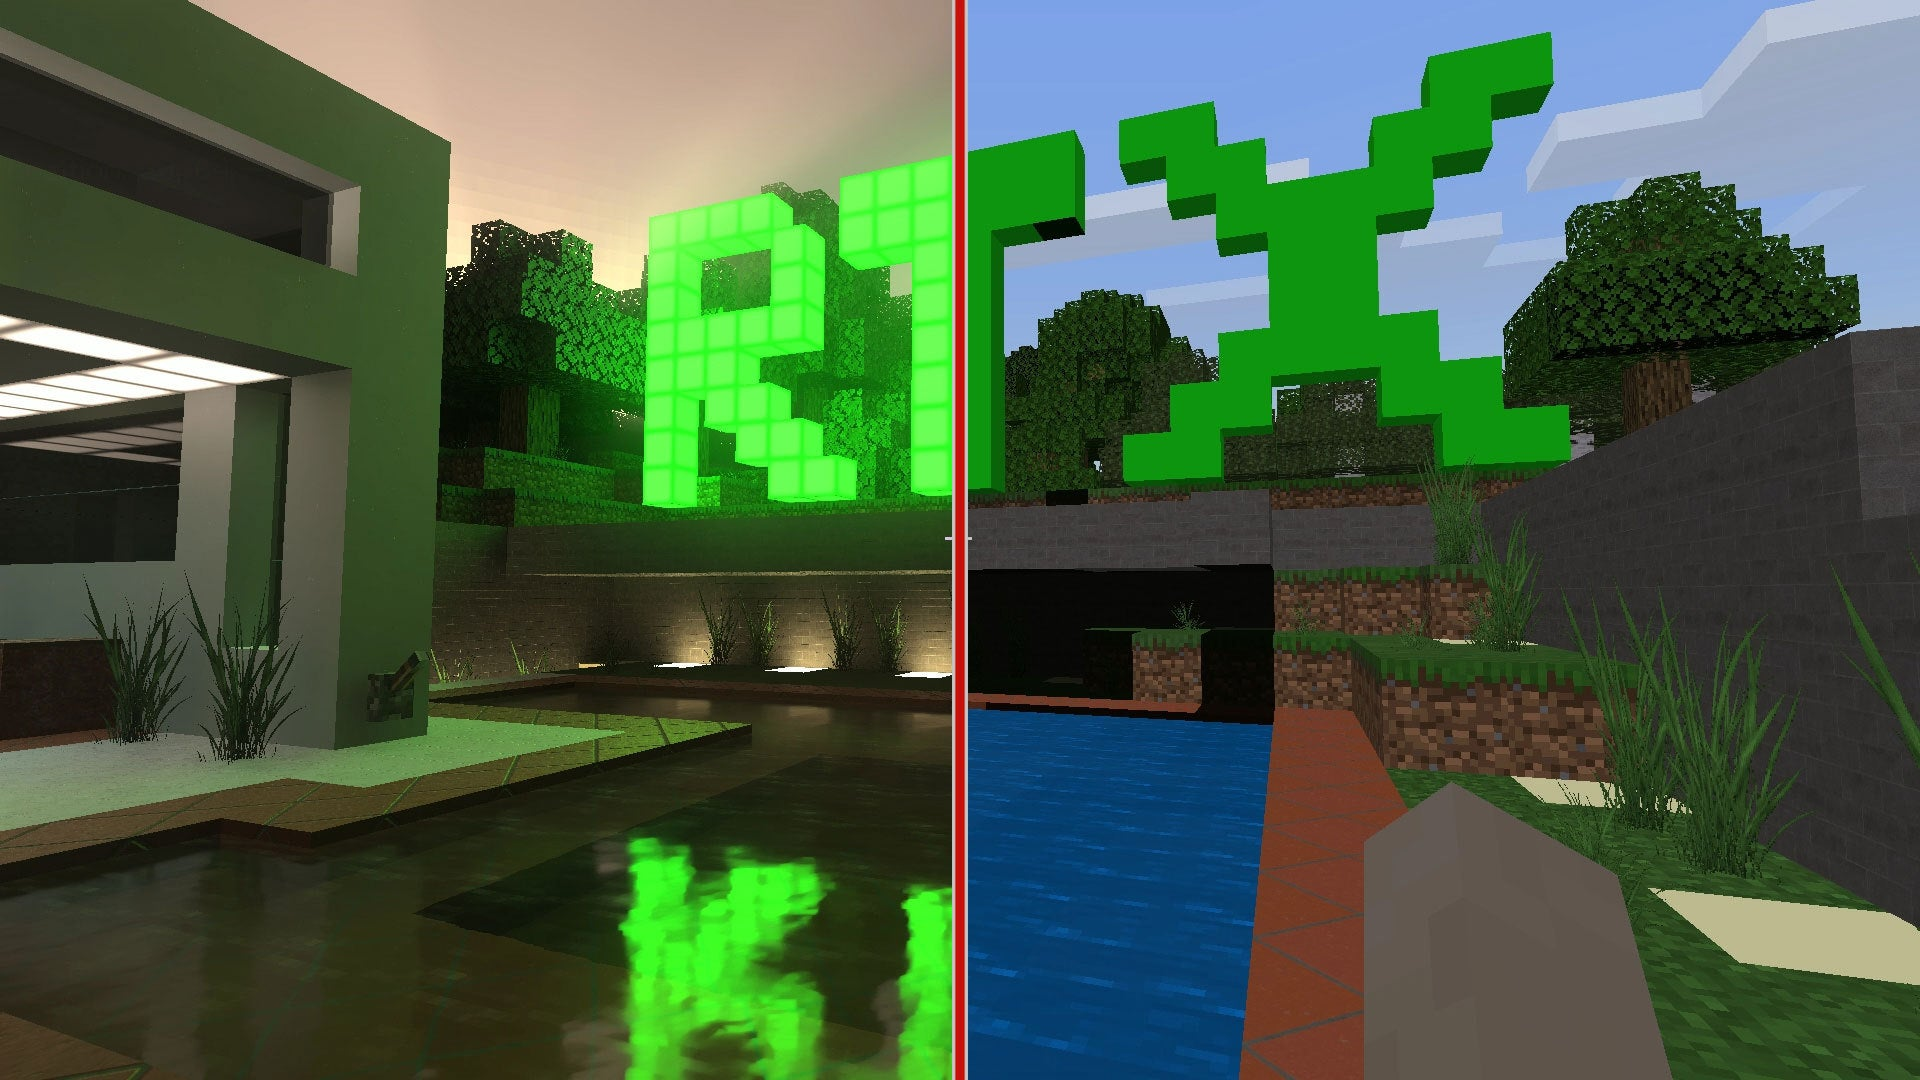
\includegraphics[width=1\textwidth]{rtx_vs_ras.jpg}
\caption{Ray tracing (left) vs. rasterization (right) \cite{comparison}}
\end{figure}
\label{image:ras_vs_rtx}
\end{center}

\chapter{Overview of Vulkan and its ray tracing extension}
While OpenGL is still continuously being updated, there is only so much that can be done for an API that is almost three decades old. This is why Vulkan was created, designed from scratch with the architecture of modern graphics cards in mind. It is a cross-platform graphics and compute API that can run on a variety of operating systems and devices. Due to all of this, Vulkan is a complex and extremely verbose API. While on the surface it might look like it is a lot more complex than OpenGL, the difference is much smaller than it appears to be. A lot of complexity (and verbosity) comes from the fact that a lot of responsibility (and by extension, control) has been shifted from the driver to the application. As a result, a hello triangle program that might have taken 20 or so lines in OpenGL 1.0 now takes over 900 lines of code in Vulkan \cite{vulkan_tutorial}.

Several key points make Vulkan more performant and suitable for modern systems than OpenGL:
\begin{itemize}
	\item Low API overhead. Instead of issuing commands to the device one by one, multiple commands are recorded to command buffers which are then submitted to the GPU.
	\item API makes no guarantees about the order of execution of commands recorded to the submitted command buffer. The application needs to use pipeline and memory barriers to create dependencies between commands. In a well-written application, this means that commands will only be blocked by the commands they depend on. This extends to other mechanisms as well, often needing explicit dependencies to be stated, giving the driver the freedom to arrange the workload in the most optimal way.
	\item API has been written with multicore CPUs in mind. While it is not possible to concurrently record commands to the same command buffer from multiple threads, it is possible to create and (concurrently) record commands to secondary command buffers which can then be tied together in a primary command buffer.
	\item Application controls memory allocations. In OpenGL, all device memory allocations are managed by the driver, whereas in Vulkan all memory allocations need to be explicitly managed by the application.
	\item Most objects in API are immutable. While this makes the API a bit more cumbersome to use, the driver can use this guarantee to make optimizations that were not possible with OpenGL.
	\item Better debugging support. Vulkan introduces the concept of validation layers - layers that can be placed between the application and the driver to ensure that calls to the API are valid and well-formed.
\end{itemize}

\section{Vulkan model overview}
\subsection{Instance and device}
The first object to be created when using Vulkan is an instance (\texttt{vk::Instance}). The application can use this object to specify which version of the API is used, enable various validation layers and define other aspects of the instance. The instance is the closest thing in Vulkan to OpenGLs global state. Once the instance has been created, physical devices can be enumerated (\texttt{vk::PhysicalDevice}), each representing specific Vulkan-compatible devices connected to the system. They can be queried for their capabilities and extension support. The next step is to create a logical device (\texttt{vk::Device}) derived out of one of the physical devices. From this point on, the logical device facilitates most of the applications communication with the API.

\subsection{Queues and command buffers}
Most of the communication between the application and the device is done via command pools (\texttt{vk::CommandPool}), command buffers (\texttt{vk::CommandBuffer}) and queues (\texttt{vk::Queue}). First, a command pool is created, connected to one of the queues available from the physical device. One or more command buffers can then be allocated from this pool. Once the commands are recorded to the command buffer, the buffer can be submitted to the queue for the device to execute.

\subsection{Synchronization}
\subsubsection{Synchronization within buffers}
All of the commands in a command buffer are executed asynchronously. Pipeline barriers act as execution barriers between various commands, ensuring that the commands are executed after the designated pipeline stages. Each pipeline barrier can reference one or more image and buffer memory barriers (\texttt{vk::ImageMemoryBarrier} and \texttt{vk::BufferMemoryBarrier}), determining the order of the operations over those resources (eg. preventing reads on a buffer or an image before all writes have been completed).

\subsubsection{Synchronization between buffers}
Submitting one command buffer before the other does not guarantee it will be executed first. On each command buffer submission, one or more binary semaphores (\texttt{vk::Semaphore}) can be supplied. The supplied semaphores are either the \linebreak semaphores that the buffer needs to wait on before executing or the semaphores that the buffer will signal once its execution is completed. Fences (\texttt{vk::Fence}) are used similarly, but they enable command buffer synchronization with the application (they are signalled by the GPU but unlike semaphores, they block CPU threads. For example, they are used to prevent the CPU from presenting the image to screen before its render is completed on the GPU. The \texttt{VK\_KHR\_TIMELINE\_SEMAPHORE} extension introduces timeline semaphores. They enable more complex dependencies to be expressed with a single semaphore holding several points in time instead of being forced to use a binary semaphore between each of the steps.

\subsection{Memory management overview}
Every Vulkan object created by the application has a handle. Once an object is created, the application has to keep track of it and destroy it once it is no longer needed. Most Vulkan objects do not need additional GPU memory other than their metadata which is handled by the driver. The two exceptions are pooled resources and application managed resources.

\subsubsection{Pooled resources}
Two examples of pooled resources are descriptor sets and command buffers. A pool object (\texttt{vk::DescriptorPool} or \texttt{vk::CommandPool}) is created from which the desired objects can then be allocated. The memory of these pools is managed by the device driver, but its amout is specified by the application.

\subsubsection{Application managed resources}
The two most notable entries of this category are buffers (\texttt{vk::Buffer}) and images (\texttt{vk::Image}). Once a handle to one of these resources is created, the application must query for the memory requirements of the object and then allocate a device memory (\texttt{vk::DeviceMemory}) with suitable properties. This memory must then be bound to the object. It is recommended to allocate a single device memory and bind several objects at various offsets, especially since it is possible to have only 4096 device memories allocated at one time (on Windows at least, Linux does not suffer from such limitations). Since most API calls that take buffers as arguments will often take both offset and size, it is possible to use a single buffer for multiple purposes. This can also be similarly done with images and image views (\texttt{vk::ImageView}), where the image view can limit access to only a part of an image.

\subsection{The swapchain and the framebuffers}
The swapchain (\texttt{vk::SwapchainKHR}) represents a set of images that can be presented to the screen. This is a rare example where the driver handles the memory allocations for an image resource. These images can be presented to a surface (\texttt{vk::SurfaceKHR}). \texttt{vk::SurfaceKHR} is an abstraction over several possible surface types, ranging from Win32 surface, all the way to Android surface. Note that both of these objects are a part of \texttt{VK\_KHR\_SWAPCHAIN} extension. Since Vulkan-capable devices can only support compute, the ability to present to a surface is not a part of the core specification but is included as an extension. When swapchain is used with the raster pipeline, each image needs to be bound to a framebuffer \linebreak (\texttt{vk::Framebuffer}). It is possible to add more than one image to the framebuffer - for example and unlike in OpenGL, the image for storing the data for the depth and stencil tests needs to be explicitly created and bound.

\subsection{The pipeline and shaders}
There are three types of pipelines (\texttt{vk::Pipeline}) in Vulkan:
\begin{itemize}
	\item{Compute pipeline}
	\item{Graphics pipeline}
	\item{Ray tracing pipeline}
\end{itemize}

Pipelines are objects that define which shaders will participate in rendering and, depending on their type, can define certain aspects of it. For example, settings on how and if triangles are culled are set in the raster pipeline. Pipelines in Vulkan are immutable, so to change almost anything in the pipeline (like swapping out a shader), a whole new pipeline needs to be constructed. Since pipeline construction is one of more time-intensive workloads in Vulkan, objects called pipeline caches (\texttt{vk::PipelineCache}) can store parts of previously constructed pipelines which are then reused when constructing new, similar pipelines. It is also advised to construct pipelines asynchronously and ahead of time.
Shaders are encapsulated in shader modules (\texttt{vk::ShaderModule}) which take a SPIR-V binary format. GLSL (and more recently HLSL) source code can be compiled to SPIR-V binary format using glslangValidator, but can also be compiled at runtime using the shaderc library. Both glslangValidator and shaderc are distributed with LunarG SDK.

\subsection{Descriptor sets and push constants}
Descriptor sets (\texttt{vk::DescriptorSet}) are the interface between the shaders and the data that to those shaders need to access. Each descriptor set has one or more bindings. Various resources can be bound to a descriptor set like samplers, images, buffers and acceleration structures (if the ray tracing extension is used). This is how materials, textures, lighting and other scene data are passed to the shaders.
Push constants are a small buffer (often only 256 bytes) that can be written directly within the command buffer (during its execution on the GPU). This is often used for a small amount of data that is constant over the length of a frame, such as view and projection matrices, or for data about the following draw call and in that case, it is updated before each new draw call.

\section{VK\_KHR\_ray\_tracing extension}
On 27th November 2018, Khronos released Vulkan revision 1.1.92.0 which introduced \texttt{VK\_NV\_ray\_tracing} extension, enabling the utilization of specialized hardware of Nvidia Turing GPUs for real-time ray tracing. Roughly a year and a half later, on 17th March 2020, Khronos released \texttt{VK\_KHR\_ray\_tracing} extension that has several advantages over the NV variant:
\begin{itemize}
	\item{The extension is vendor-neutral, making it more likely for vendors other than Nvidia to support it.}
	\item{Extension offers more flexibility in building acceleration structures.}
\end{itemize}

At the time of writing this paper, the KHR variant of the extension was still in beta.

The extension itself introduces several new concepts to Vulkan:
\begin{itemize}
	\item{Acceleration structures}
	\item{Ray tracing shaders}
	\item{Shader binding table}
	\item{Ray tracing pipeline}
\end{itemize}

\subsection{Acceleration structures}
Acceleration structures (\texttt{vk::AccelerationStructure}) are objects used to accelerate ray tracing. Instead of testing each ray for intersection with every triangle in the scene, a BVH that reduces the complexity of the search from O(n) to O(logn). There are two types of acceleration structures in the API. Bottom level acceleration structures (BLAS) can hold one or more geometries. Each geometry consists of a list of vertices which can be indexed. Top level acceleration structures (TLAS) reference BLASes. Each instance of BLAS is given a unique identifier and transformation (even if it references the same BLAS) which is later available in the shader. This enables the ray tracing equvivalent of rasterization model instancing.

Acceleration structures are usually built on the GPU, but with the new extension, they can now be built on the CPU and uploaded to the GPU later. In cases where GPU is under a heavy load while the CPU has one or more cores idle, acceleration structure can be built on those cores instead, balancing the workload between the GPU and the CPU.

The actual process of building the acceleration structure is handled by the driver. The driver can be instructed to build the structure with ray tracing speed or speed of the build itself being prioritized. Acceleration structures, if so specified during their creation, can also be updated, which is faster than rebuilding them. Not all acceleration structures are suitable for updates - where a tree with branches swaying in the wind would be an example of a good acceleration structure to update, while one depicting an object which is exploding would not.

\subsection{Ray tracing shaders}
This extension introduces several new shader types:
\begin{itemize}
	\item{Ray generation shader}
	\item{Any hit shader}
	\item{Closest hit shader}
	\item{Miss shader}
	\item{Intersection shader}
	\item{Callable shader}
\end{itemize}

Since the shaders themselves are not a part of Vulkan API, but SPIR-V specification, they are introduced through a SPIR-V extension \texttt{SPV\_KHR\_ray\_tracing}.

\subsubsection{Ray generation shader}
Ray tracing pipeline is entered similarly to a compute pipeline. A workload is submitted in three dimensions. The first two dimensions are most often used as screen dimensions in pixels, while the third one is usually set to 1, or can be used as a number of samples per pixel. For each 3D coordinate, a ray generation shader is invoked. The most common uses of this shader are to calculate the trajectory of the ray passing through the designated pixel, invoke ray tracing (\texttt{traceRayEXT} function) and write the result to an image. Segment of the ray that the tests will be performed on has to be defined, serving a purpose similar to the far and near planes of the scene frustum.

\subsubsection{Any hit shader}
Once \texttt{traceRayEXT} is invoked, the hardware tests for intersections between the triangles of the TLAS and the ray. This shader is invoked for each triangle hit. It is advised to keep these shaders short and fast since they get invoked many times per ray. This shader is optional and need not be implemented.

\subsubsection{Closest hit shader}
This shader is invoked over the closest intersection found in all of the geometry stored in the provided TLAS.

\subsubsection{Miss shader}
This shader is invoked if no intersection is found between the TLAS and the ray. This can be used to sample a cube map to render a skybox around the scene or to signal that there is no obstruction between the ray origin and the ray target, which is very useful for shadow testing.

\subsubsection{Intersection shader}
While the geometry is usually defined as a set of triangles, it can also be defined as a set of 3D objects, as long as they can fit within an axis-aligned bounding boxes (AABB). If that is the case, the testing will be done against the AABBs and the intersection shader will be invoked on a hit, enabling calculations determining if and how the ray hits the bounded object. This shader is required only if TLAS contains a BLAS whose geometry type is AABB.

\subsubsection{Callable shader}
Callable shaders are shaders that can be called from other programmable shaders. Due to the parallelism of the GPU, the driver is able to better optimize such calls opposed to if functions within the shaders are invoked.

\subsection{Shader binding table}
With standard rasterization, various objects with different properties can be rendered one after another, swapping the shaders in and out as needed. When it comes to ray tracing, the ray can hit any object in the scene, requiring all of the shaders to be available at the same time. The shader binding table holds the handles to every shader that can be invoked during the ray tracing process. The handles are divided into groups. Ray generation shader and miss shaders are each in their own separate groups, while any hit shaders and closest hit shaders form hit groups. Shader binding table is referenced in two contexts - firstly, when initially invoking the ray generation shaders from within the command buffer and secondly, from within shaders for recursive ray tracing.

\subsection{Ray tracing pipeline}
Ray tracing pipeline is quite a bit simpler than it's raster counterpart since there is not much to set up. Its main use is to bind the various shaders and groups into a single object.


\chapter{Implementation of a simple ray traced application}
The goal is to create an application that renders a voxelized space. The application can be run in two configurations:
\begin{itemize}
	\item using a raster pipeline
	\item using a ray tracing pipeline
\end{itemize}

Raster pipeline has been developed first to be used as a baseline and to compare it's performance to the performance of the ray tracing pipeline.

The application can be divided into three main parts:
\begin{itemize}
	\item{Generation and meshing of chunks}
	\item{Rasterizer}
	\item{Ray tracer}
\end{itemize}

\section{Generation and meshing of the chunks}
This part of the application has mostly been covered in chapter 3. Each block in the chunk can either be a completely transparent air block or a completely opaque solid block. Application can be customised by defining the dimensions of a chunk (NxNxN, all dimensions are the same), the number of chunks that will be rendered (MxMx1, all chunks are laid on the same XZ plane) and the percentage of the chunk that is solid. For this example, each chunk is 32x32x32 blocks in size, there are 32x32x1=1024 chunks and 10\% of the chunks are solid blocks. The chunks are generated in three steps:
\begin{itemize}
	\item{A vertex array is created, containing each of 33x33x33=35,937 possible vertex positions. A single array is used for all of the chunks.}
	\item{For each chunk, a three dimensional array is filled with random values: \linebreak \texttt{blocks[i][j][k] = rand() \% 10 == 0;}}
	\item{Greedy meshing algorithm is executed for each chunk, creating an index array for each one}
\end{itemize}

An additional optimization has been made to the greedy mesher - each set of parallel slices is generated in a separate thread.

The vertex and all of the index arrays are then copied to the GPU.

\section{Rasterizer}
When raster pipeline configuration is selected, Phong shading with a single point light is used to shade all of the blocks. The result can be seen in image \ref{image:raster}.

\begin{center}
\begin{figure}[H]
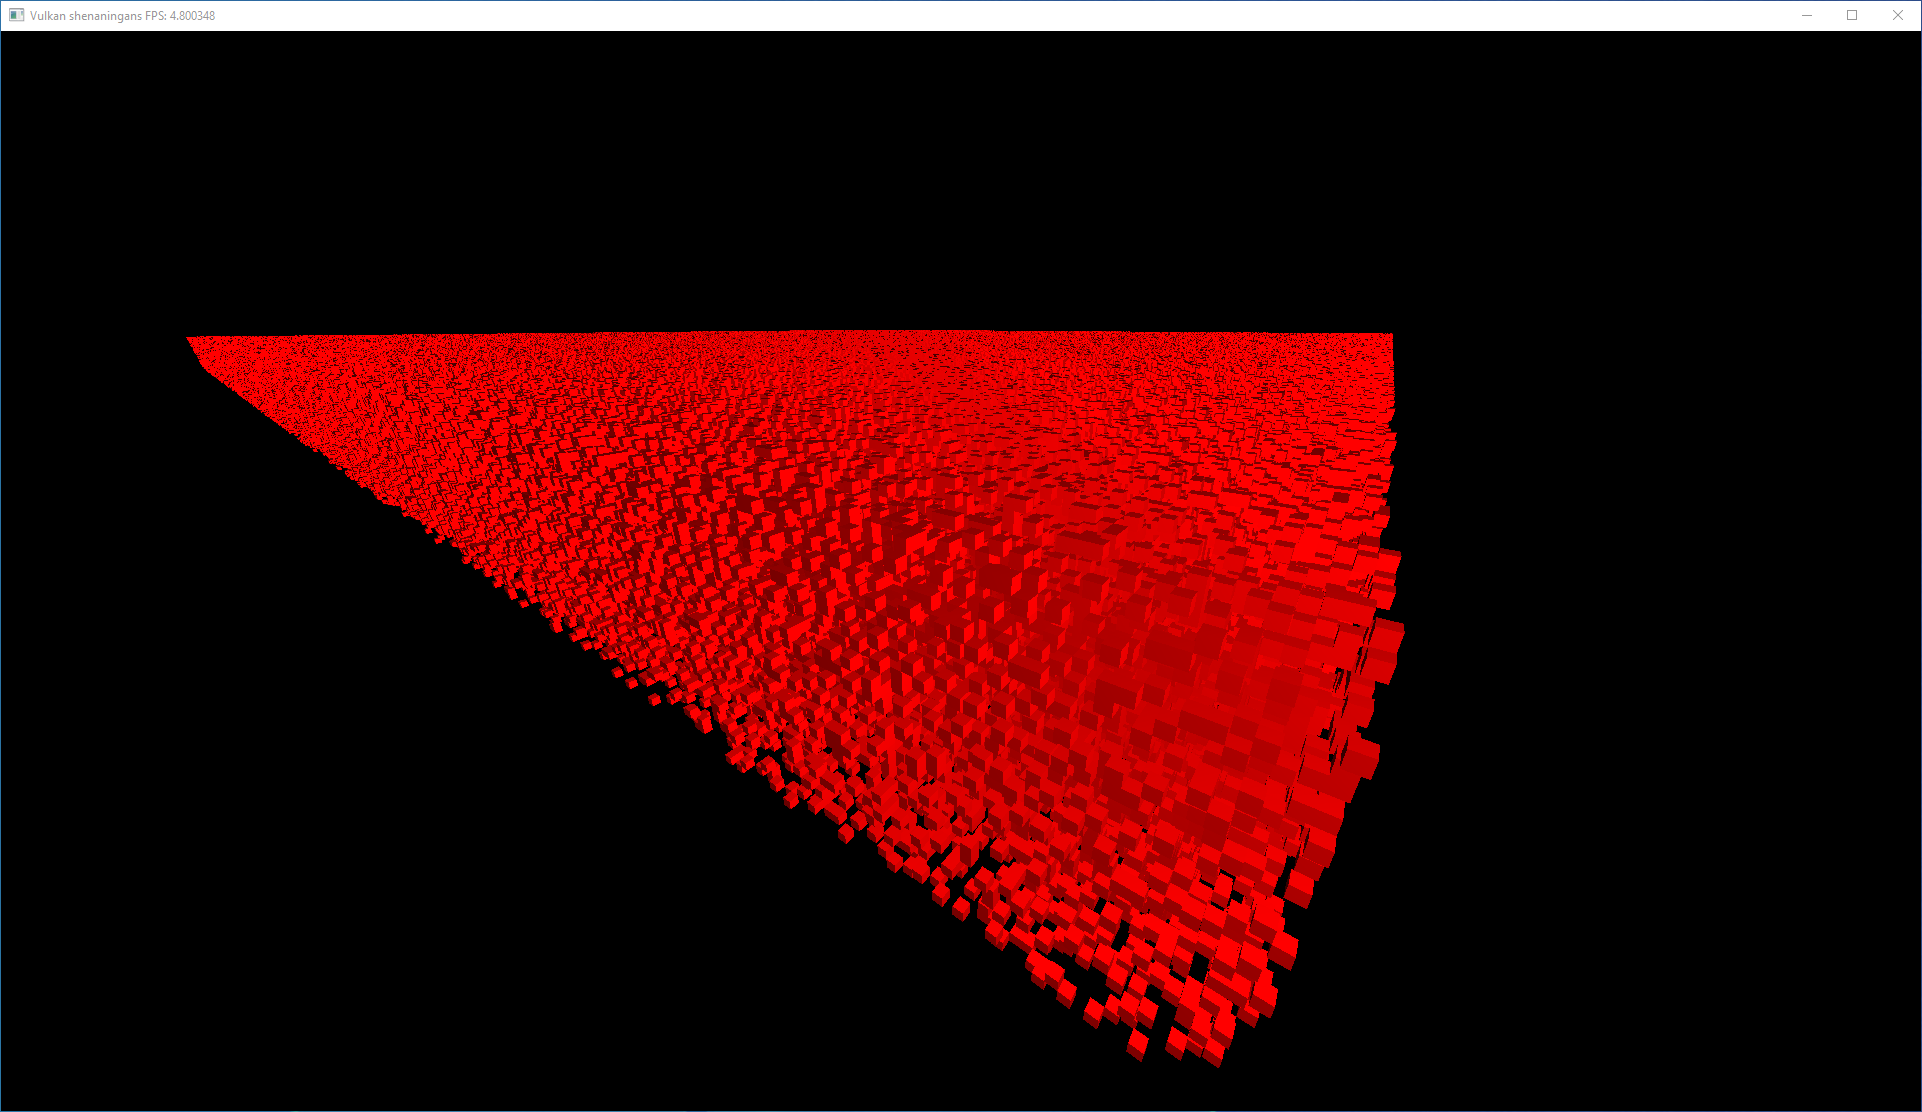
\includegraphics[width=1\textwidth]{raster.png}
\caption{Rasterized image with a single point light}
\label{image:raster}
\end{figure}
\end{center}

\section{Ray tracer}
When the application is run in the ray tracing configuration, a complete ray tracing pipeline is setup. The shaders are setup to demonstrate smooth shadows and perfect reflections (image \ref{image:ray_traced}), two effects that are very difficult to achieve solely with a raster pipeline. The following data is made available to the shaders:
\begin{itemize}
	\item{the acceleration structure}
	\item{storage image as the render target}
	\item{the vertex buffer}
	\item{an array of index buffers, one per chunk}
	\item{an array of sample sets used when sampling the light source in shadow testing}
	\item{view and projection matrices, camera position and definition of the light source}
\end{itemize}

\begin{center}
\begin{figure}[H]
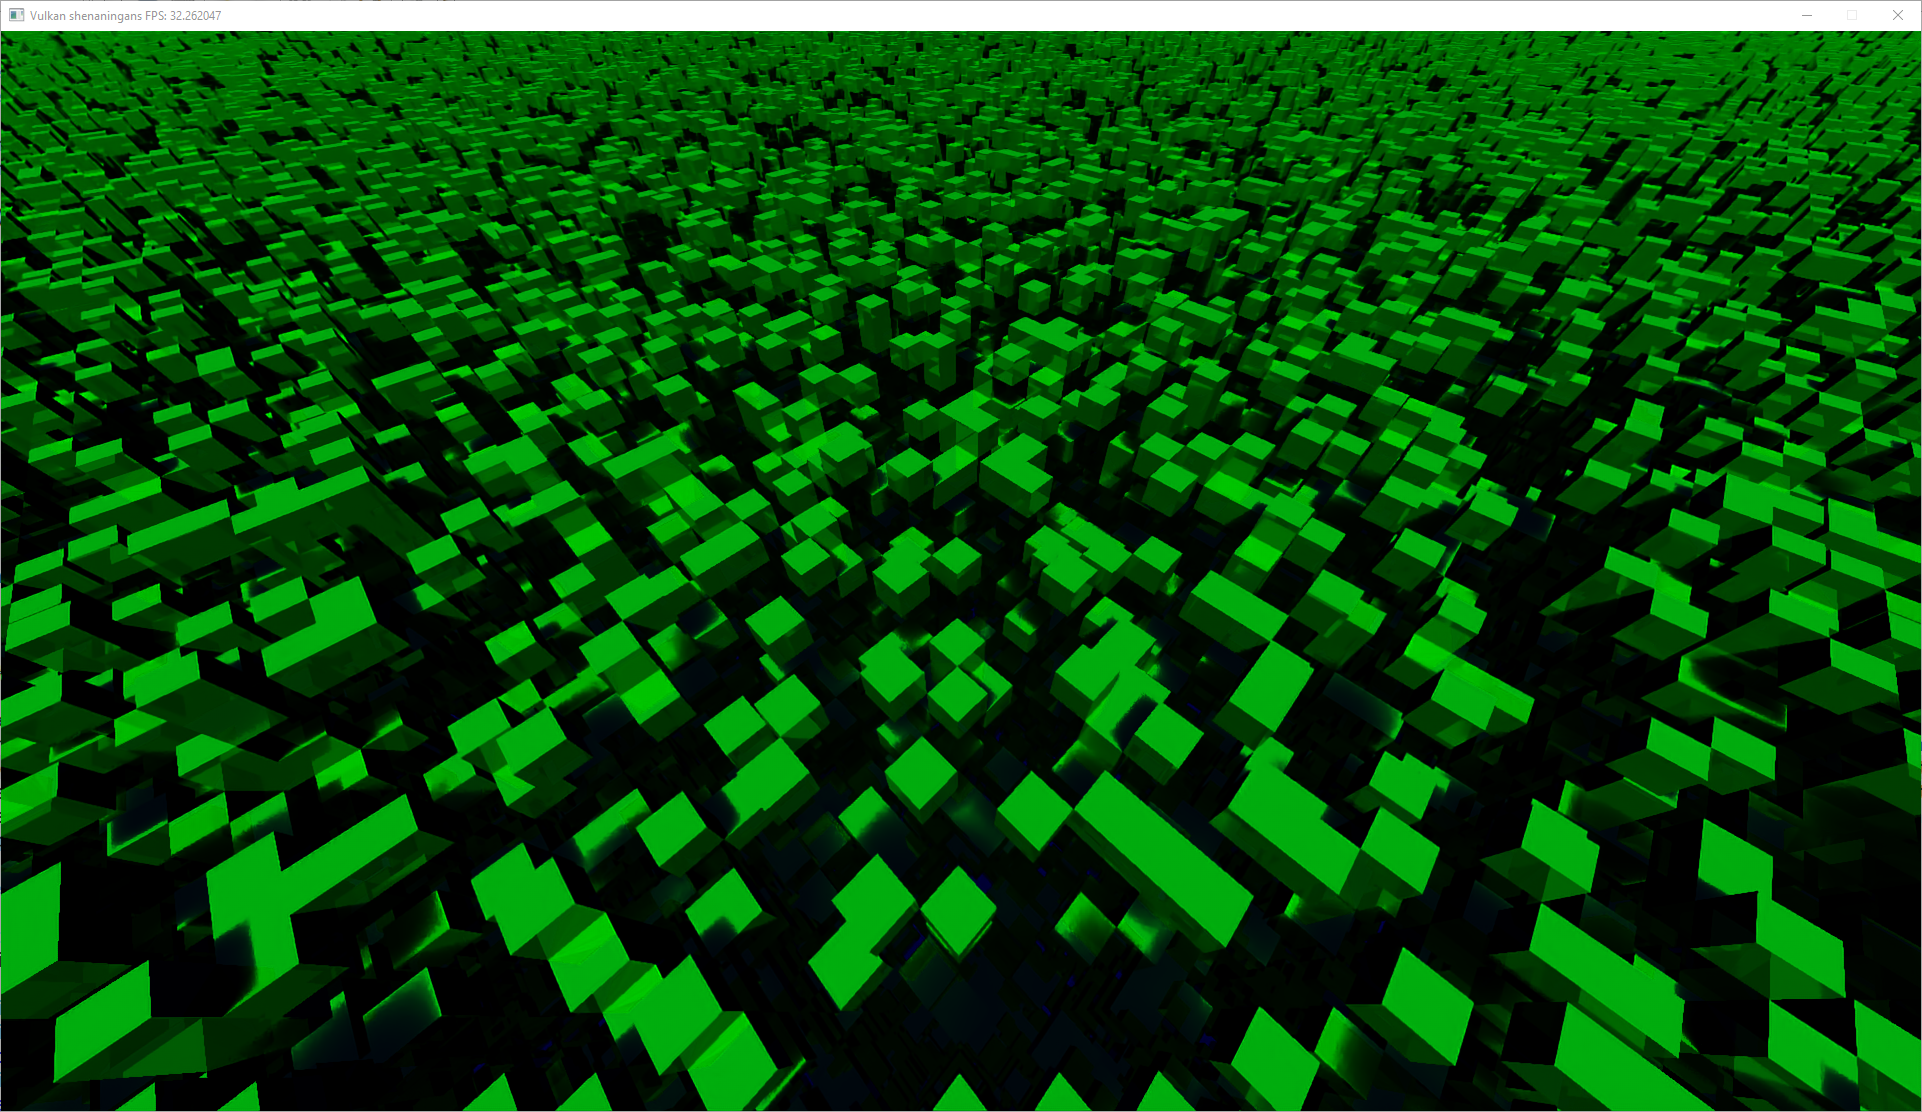
\includegraphics[width=1\textwidth]{ray_trace.png}
\caption{Ray traced image with a single area light, reflections and shadows}
\label{image:ray_traced}
\end{figure}
\end{center}

\begin{lstlisting}[language=c++, style=cppstyle, caption=Closest hit shader used in the application, frame=single]
#version 460
#extension GL_EXT_ray_tracing : enable
#extension GL_EXT_scalar_block_layout : enable
#extension GL_EXT_nonuniform_qualifier : enable

hitAttributeEXT vec3 attribs;

struct Payload {
    vec3 hitValue;
    uint depth;
};

layout(location = 0) rayPayloadInEXT Payload backPayload;

layout(location = 1) rayPayloadEXT bool isShadowed;
layout(location = 2) rayPayloadEXT Payload forwardPayload; 

struct Vertex {
    vec3 pos;
};

layout(binding = 0, set = 0) uniform accelerationStructureEXT
    topLevelAS;
layout(binding = 2, set = 0, scalar) uniform UniformBuffer 
{
    vec3 lightSpan[4];
    uint reflectionsEnabled;
    uint shadowsEnabled;
} UB;

layout(binding = 3, set = 0, scalar) buffer Vertices {
    Vertex v[];
} vertices;

layout(binding = 4, set = 0) buffer Indices {
    uint i[];
} indices[];

layout(binding = 5, set = 0) buffer Sample {
    vec2 samplePoints[];
} sampleSets[];

layout( push_constant ) uniform PushConstants {
    mat4 viewInverse;
    mat4 projInverse;
    vec3 cameraPosition;
} push;

float PHI = 1.61803398874989484820459; // Golden Ratio   
float goldNoise(in vec2 xy, in float seed){
       return fract(tan(distance(xy*PHI, xy)*seed)*xy.x);
}

vec3 sampleValue(vec3 a, vec3 b, vec3 c, vec2 offset) {
    vec3 abDir = (b-a) * offset.x;
    vec3 acDir = (c-a) * offset.y;

    return a + abDir + acDir;
}

void main()
{
    if (backPayload.depth == 0) {
        return;
    }

    ivec3 ind = ivec3(
        indices[gl_InstanceCustomIndexEXT].i[3 * gl_PrimitiveID + 0],
        indices[gl_InstanceCustomIndexEXT].i[3 * gl_PrimitiveID + 1],
        indices[gl_InstanceCustomIndexEXT].i[3 * gl_PrimitiveID + 2]);

    vec3 v0 = vertices.v[ind.x].pos;
    vec3 v1 = vertices.v[ind.y].pos;
    vec3 v2 = vertices.v[ind.z].pos;

    vec3 first = v1 - v0;
    vec3 second = v2 - v0;
    vec3 normal = normalize(cross(first, second));

    vec3 worldPos =
        gl_WorldRayOriginEXT
        + gl_WorldRayDirectionEXT * gl_HitTEXT;

    if (dot(normal, worldPos - push.cameraPosition) > 0) {
        backPayload.hitValue = vec3(0.0f);
        return;
    }

    vec3 toLight[4];
    toLight[0] = normalize(UB.lightSpan[0] - worldPos);
    toLight[1] = normalize(UB.lightSpan[1] - worldPos);
    toLight[2] = normalize(UB.lightSpan[2] - worldPos);
    toLight[3] = normalize(UB.lightSpan[3] - worldPos);

    float lightAngle[4];
    lightAngle[0] = dot(normal, toLight[0]);
    lightAngle[1] = dot(normal, toLight[1]);
    lightAngle[2] = dot(normal, toLight[2]);
    lightAngle[3] = dot(normal, toLight[3]);

    float shadowFactor = 1;
    if (UB.shadowsEnabled == 1 &&
        (lightAngle[0] > 0
        || lightAngle[1] > 0
        || lightAngle[2] > 0
        || lightAngle[3] > 0)) {

        float tMin = 0.001;
        vec3 origin = worldPos;
        uint flags = 
            gl_RayFlagsTerminateOnFirstHitEXT
            | gl_RayFlagsOpaqueEXT
            | gl_RayFlagsSkipClosestHitShaderEXT;

        uint obstruction = 0;
        uint shadowSampleCount = 25;

        uint index = int(
            100
            * goldNoise(
                worldPos.xy * worldPos.zy,
                worldPos.z + worldPos.x)
       );

        for (uint i = 0; i < shadowSampleCount; ++i) {
            vec3 samplePoint = sampleValue(
                UB.lightSpan[0],
                UB.lightSpan[1],
                UB.lightSpan[2],
                sampleSets[index].samplePoints[i]
            );

            float tMax = length(samplePoint - worldPos);
            vec3 rayDir = normalize(samplePoint - worldPos);
            isShadowed = true;
            traceRayEXT(
                topLevelAS,
                flags,
                0xFF,
                0,
                0,
                1,
                origin,
                tMin,
                rayDir,
                tMax,
                1);

            if (isShadowed) {
                ++obstruction;
            }
        }

        shadowFactor = 1.0 / (1 + obstruction);
    }

    float diffuseFactor = (
        lightAngle[0]
        + lightAngle[1]
        + lightAngle[2]
        + lightAngle[3]
    ) / 4.0;

    vec3 lightBase =
        shadowFactor
        * diffuseFactor
        * vec3(0.0f, 1.0f, 0.0f);

    vec3 toEye = normalize(push.cameraPosition - worldPos);
    vec3 reflectedToEye = -toEye - 2 * dot(normal, -toEye) * normal;

    forwardPayload.hitValue = vec3(0.0f);
    forwardPayload.depth = backPayload.depth - 1;

    if (UB.reflectionsEnabled == 1) {
        traceRayEXT(
            topLevelAS,
            gl_RayFlagsOpaqueEXT,
            0xFF,
            0,
            0,
            0,
            worldPos,
            0.001,
            reflectedToEye,
            1000.0,
            2);
    }

    backPayload.hitValue =
        0.75 * lightBase
        + 0.25 * forwardPayload.hitValue;
}
\end{lstlisting}

In the ray generation shader, a single primary ray per pixel is traced. When the closest intersection with the ray is found, triangle ID, index array and vertex array are used to determine the vertices and the normal of the triangle. The light source is modelled as four coplanar points describing a rectangle. A dot product is calculated between the normal of the hit triangle and vectors going from the intersection towards each of the light corners. If at least one of the results is positive, a shadow test is performed.
The shadow test involves picking one of the sample sets from the array. The samples are generated using multi-jittered sampling \cite{ray_tracing} on a unit rectangle. This is then superimposed over the light source and, in this case, 25 samples are chosen. A ray is traced from the intersection towards each of the samples and the shadow factor is determined as a number of samples over (1 + number of obstructed samples). The diffuse factor is calculated as an average of the dot product between the hit triangle normal and the vector towards each of the corners of the light source. The shadow factor and the diffuse factor are then multiplied with the colour of the triangle (in this case, solid green) to get the base colour. If reflections are enabled, a new reflected ray is traced from the intersection, repeating the whole process recursively up to a predefined depth. On each layer of the recursion, the base colour of the current layer and the base colour of the layer deeper in the recursion are combined in a ratio 3:1.

Once the resulting image is produced, if denoising is enabled, the image is sent to the denoiser for post-processing. Either way, the image is then copied to the swapchain and presented to the screen.

\section{Performance measurements}
In this chapter, multiple application configurations are tested and compared. All of the tests are run on a machine with specifications described in table ~\ref{table:specifications}.

\begin{table}[H]
\begin{center}
\caption{Specifications of the test machine}
\begin{tabular}{|c|c|}
\hline
Component type & Component used \\
\hline
CPU & Intel Core i9-9900KS \\
\hline
GPU & Nvidia GeForce RTX 2080Ti \\
\hline
RAM & 32GB DDR4 3600CL16 \\
\hline
\end{tabular}
\label{table:specifications}
\end{center}
\end{table}

The same scene is used for each test. It consists of 1024 32x32x32 chunks arranged in a 32x32x1 pattern. 10\% of each chunk is randomly filled with opaque blocks, but the seed is set at the start of the program, so the same scene consisting of 30,917,848 triangles is generated on every run. Resolution is set to 1920x1080.

It takes roughtly 20 seconds for the application to start rendering in both raster and render mode since about 80\% of initialization time is spent on meshing the chunks.

Performance is calculated as an average frame time over a period of 5 seconds after the application has been initialized. The camera is not moved during that period. The frame time includes workloads on both the CPU and the GPU.

The first test is a comparison between the raster (image \ref{image:raster_simple}) and ray tracing (image \ref{image:ray_trace_simple}) pipelines, the results can be viewed in table ~\ref{table:ras_vs_ray}. There are no calculations in the shaders, if a block is present, the pixel is coloured in a solid colour. Since the program has to be recompiled to change the rendering technique, the camera is positioned in the roughly the same position and orientation. The whole scene is visible in the frame.

\begin{table}[H]
\caption{Rasterization vs. ray tracing}
\begin{center}
\begin{tabular}{|c|c|}
\hline
Test & Average frame time \\
\hline
Rasterization & ~4.37ms \\
\hline
Ray tracing & ~1.13ms \\
\hline
\end{tabular}
\label{table:ras_vs_ray}
\end{center}
\end{table}

Ray tracing is almost four times faster than rasterization. This result is unexpected, especially since the implementation of the ray tracing pipeline is less parallel than the rasterization one. Another contributing factor could be that a new value is written to the push constants before every chunk is written, something that can add up with 1024 chunks being rendered.

\begin{center}
\begin{figure}[H]
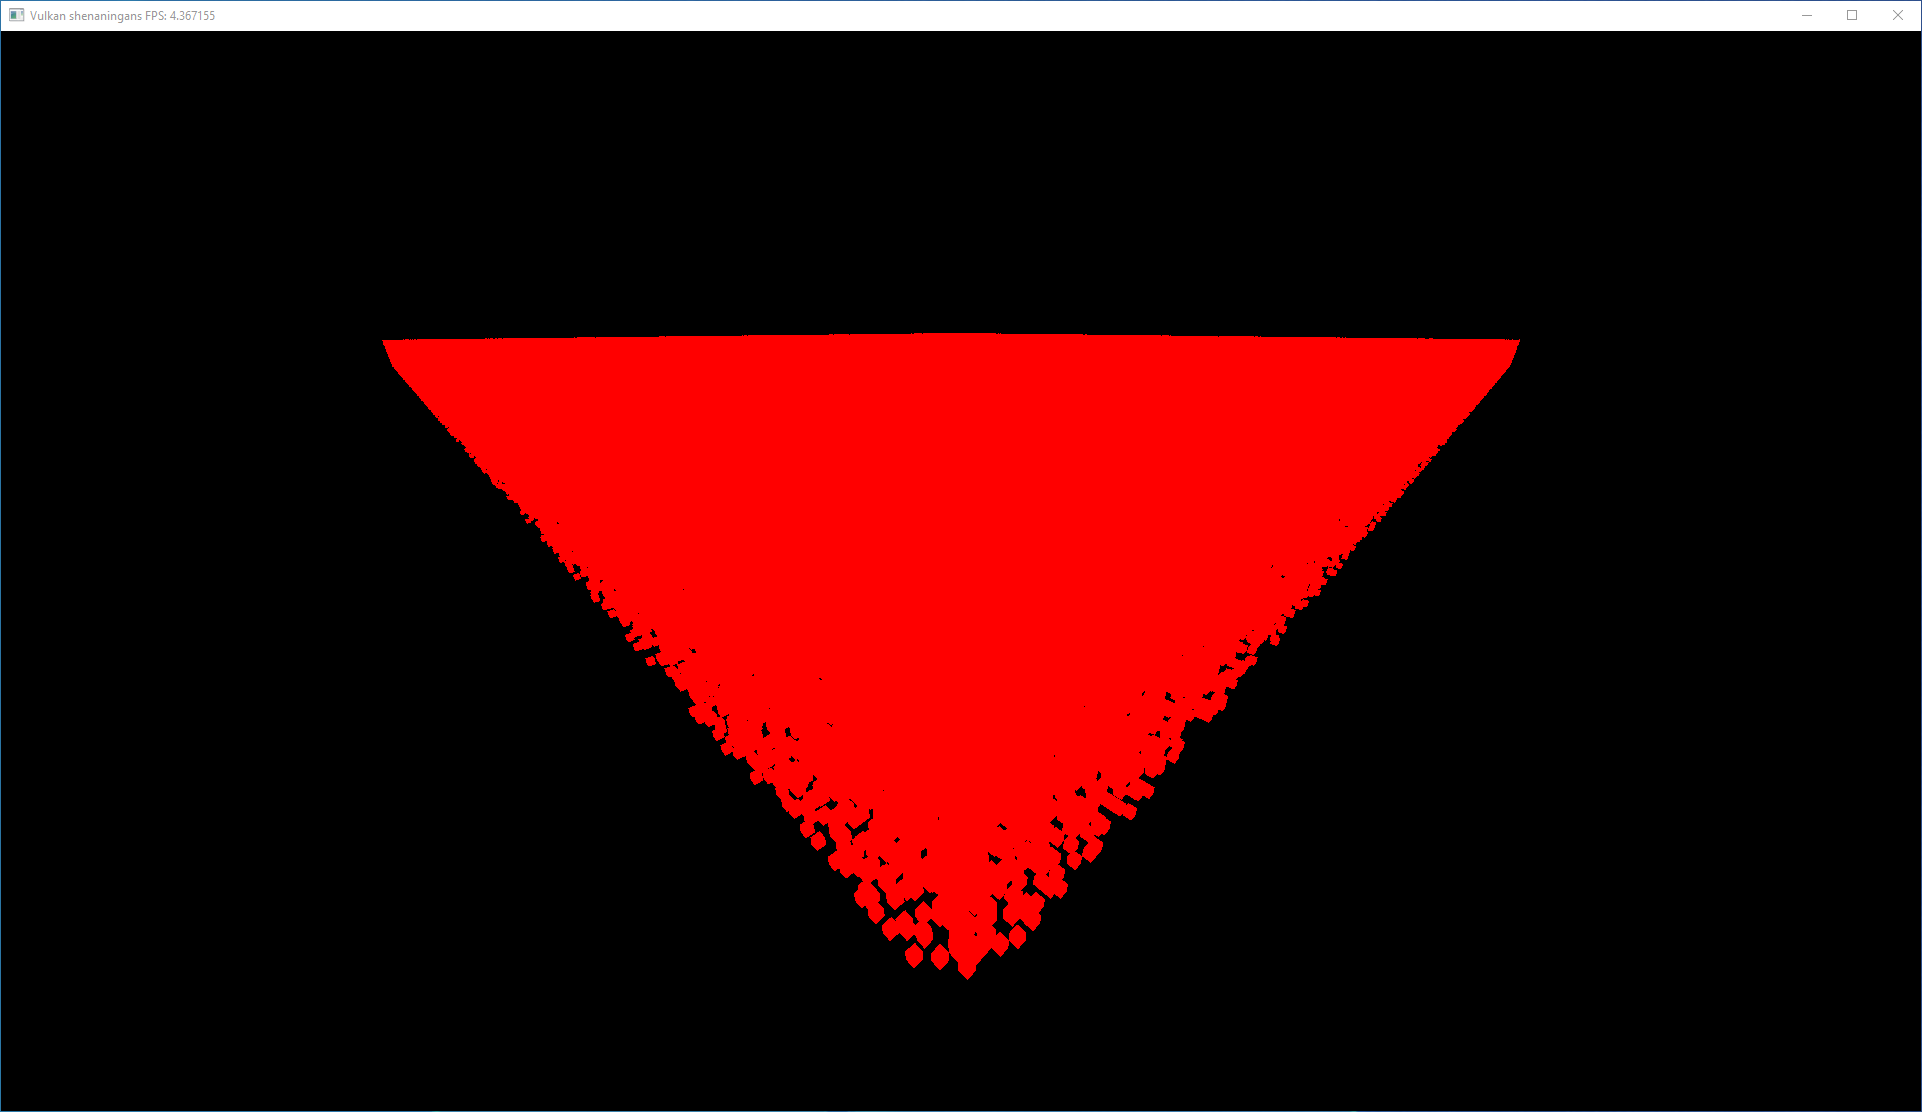
\includegraphics[width=1\textwidth]{tests/raster_simple.png}
\caption{Resulting image when rasterization is used}
\label{image:raster_simple}
\end{figure}
\end{center}

\begin{center}
\begin{figure}[H]
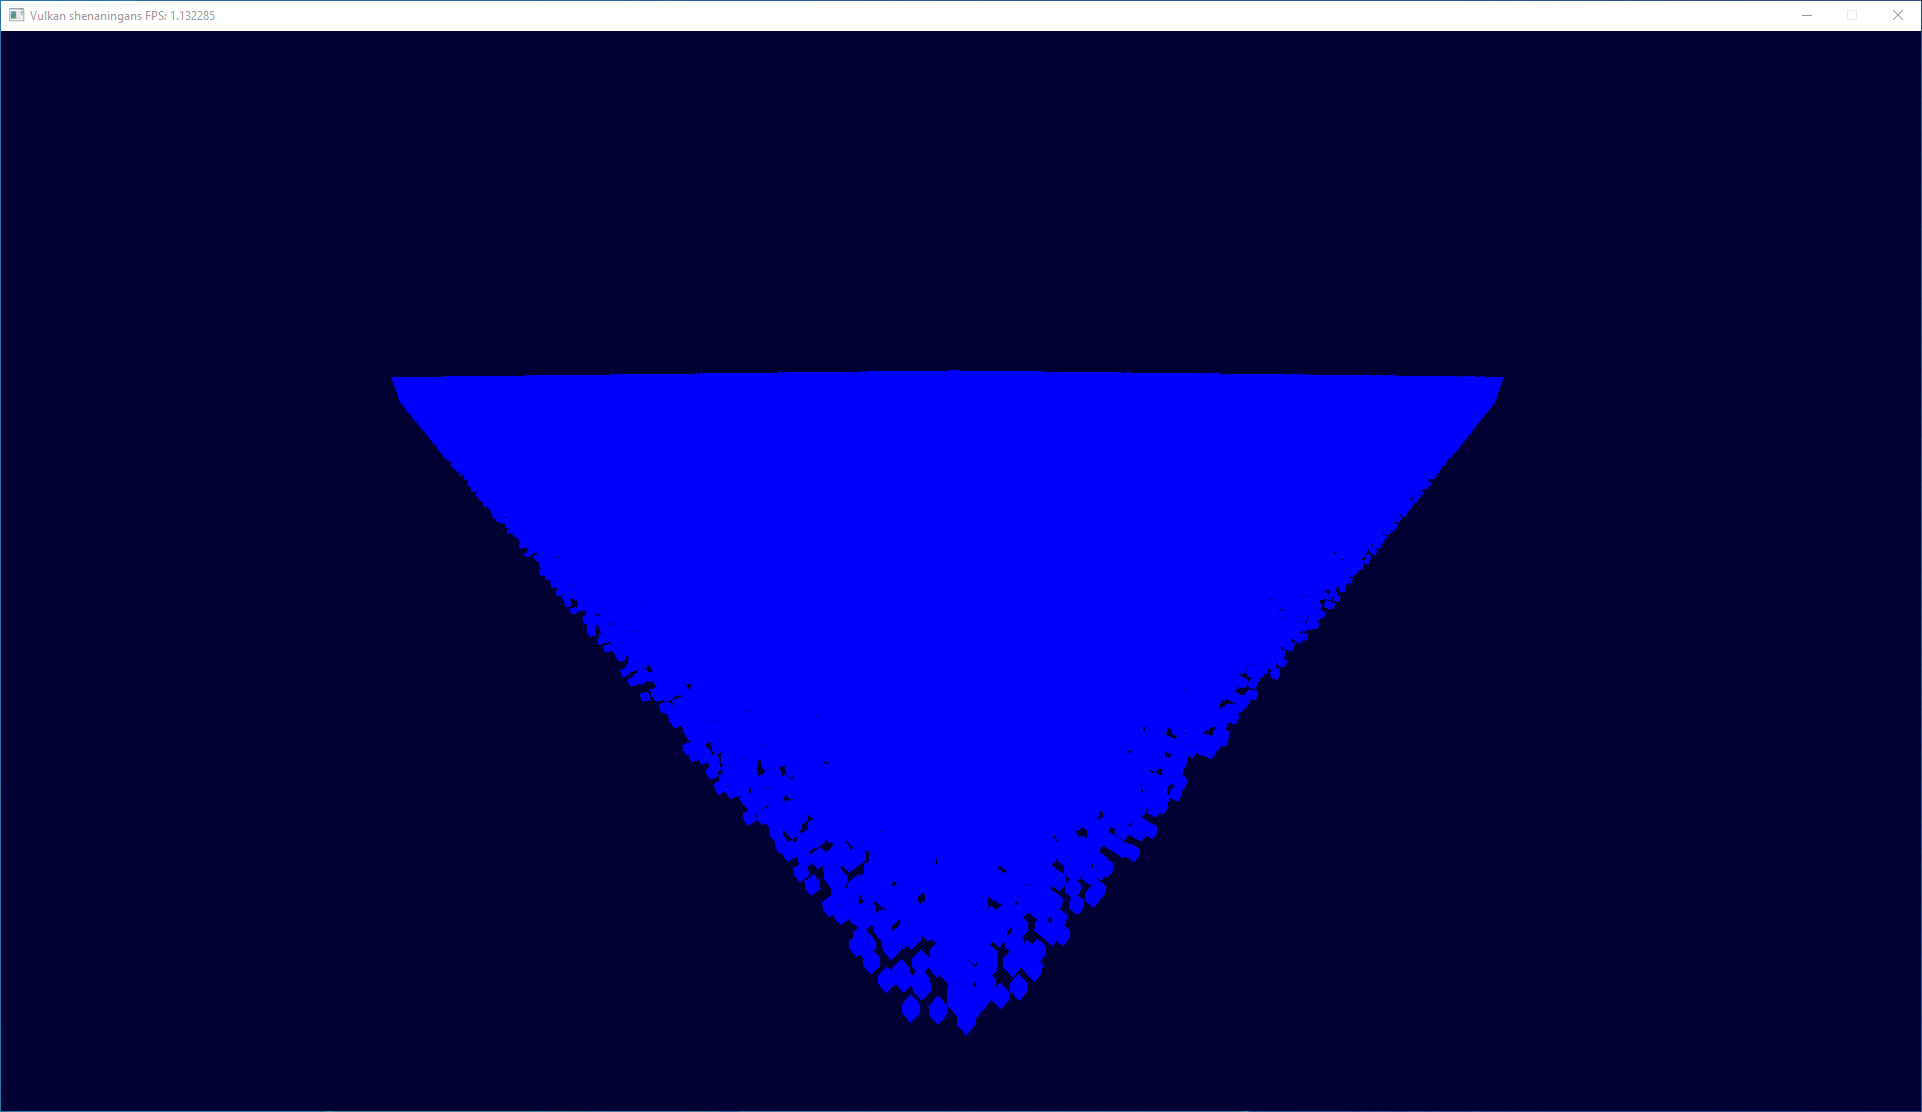
\includegraphics[width=1\textwidth]{tests/ray_trace_simple.png}
\caption{Resulting image when ray tracing is used}
\label{image:ray_trace_simple}
\end{figure}
\end{center}

The following tests compare the impact of shadows, reflections and denoising on the frame times, the results are in table ~\ref{table:real_test}. All of these features can be toggled during runtime, so each test is run on exactly the same frame.
Reflections are set to 5 bounces, while shadows are calculated using 25 samples.
\begin{table}[H]
\caption{Rasterization vs. ray tracing}
\begin{center}
\begin{tabular}{|c|c|}
\hline
Test & Average frame time \\
\hline
All off & ~1.00ms \\
\hline
Reflections only & ~2.09ms \\
\hline
Shadows only & ~8.14ms \\
\hline
Denoising only & ~16.47ms \\
\hline
Reflections + denoising & ~17.83ms \\
\hline
Shadows + reflections & ~19.12ms \\
\hline
Shadows + denoising & ~23.30ms \\
\hline
All on & ~34.82ms \\
\hline
\end{tabular}
\label{table:real_test}
\end{center}
\end{table}

Reflections seem to have a lower impact on performance than shadows since reflections trace only 5 additional rays per primary ray, opposed to shadows which trace 25. Denoising seems to impact performance quite a lot, especially when combined with other effects, especially shadows. Since the sole purpose of denoising is to smooth out the shadows in the scene, there is not much point in turning denoising on if no (smooth) shadows are present. It is also worth noting that reflections decrease the quality of the denoised image. Since the shadowed surface is no longer of a solid colour, the denoiser has additional data for which it has no way of filtering out. Using the earlier mentioned advanced version of the denoiser with the additional input could improve the quality of the result. Resulting renders can be seen in images \ref{image:all_off} to \ref{image:all_on} 

\begin{center}
\begin{figure}[H]
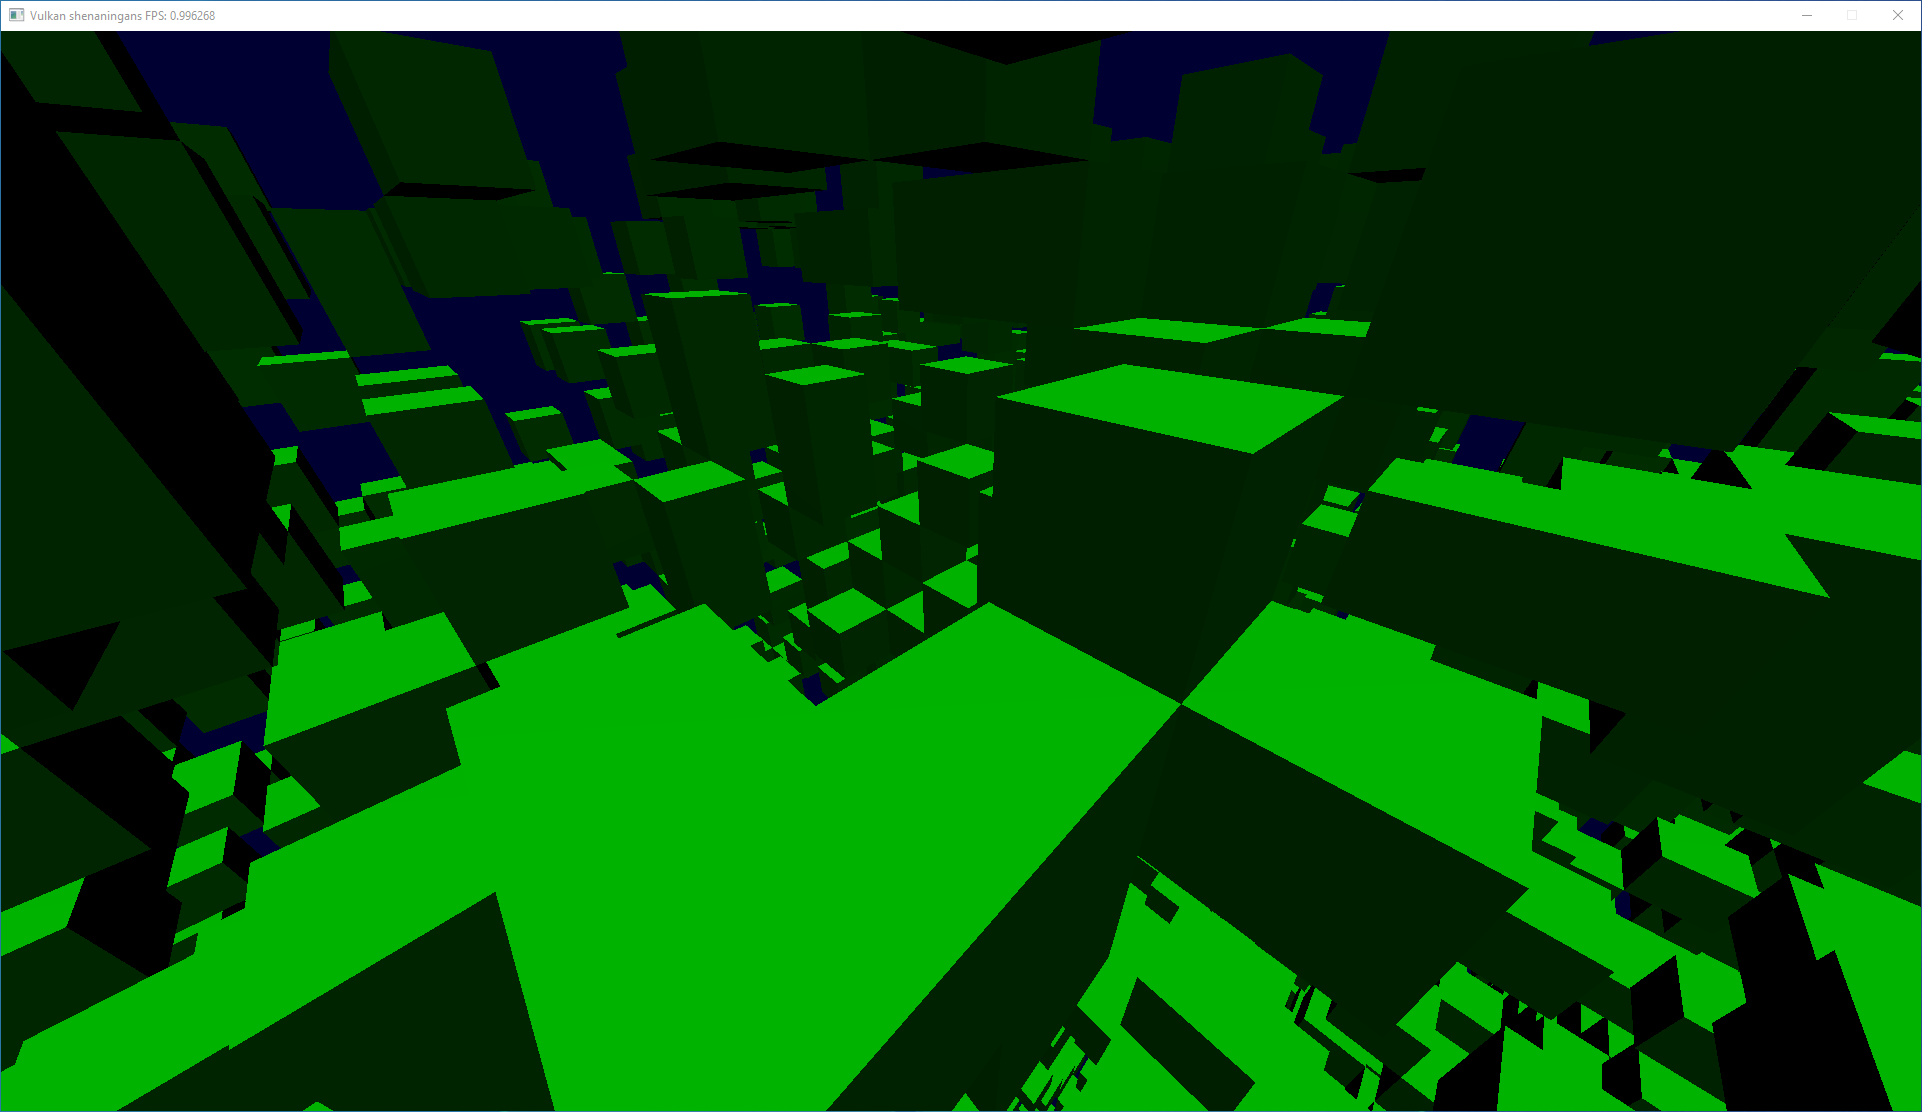
\includegraphics[width=1\textwidth]{tests/all_off.png}
\caption{Test with all features disabled}
\label{image:all_off}
\end{figure}
\end{center}

\begin{center}
\begin{figure}[H]
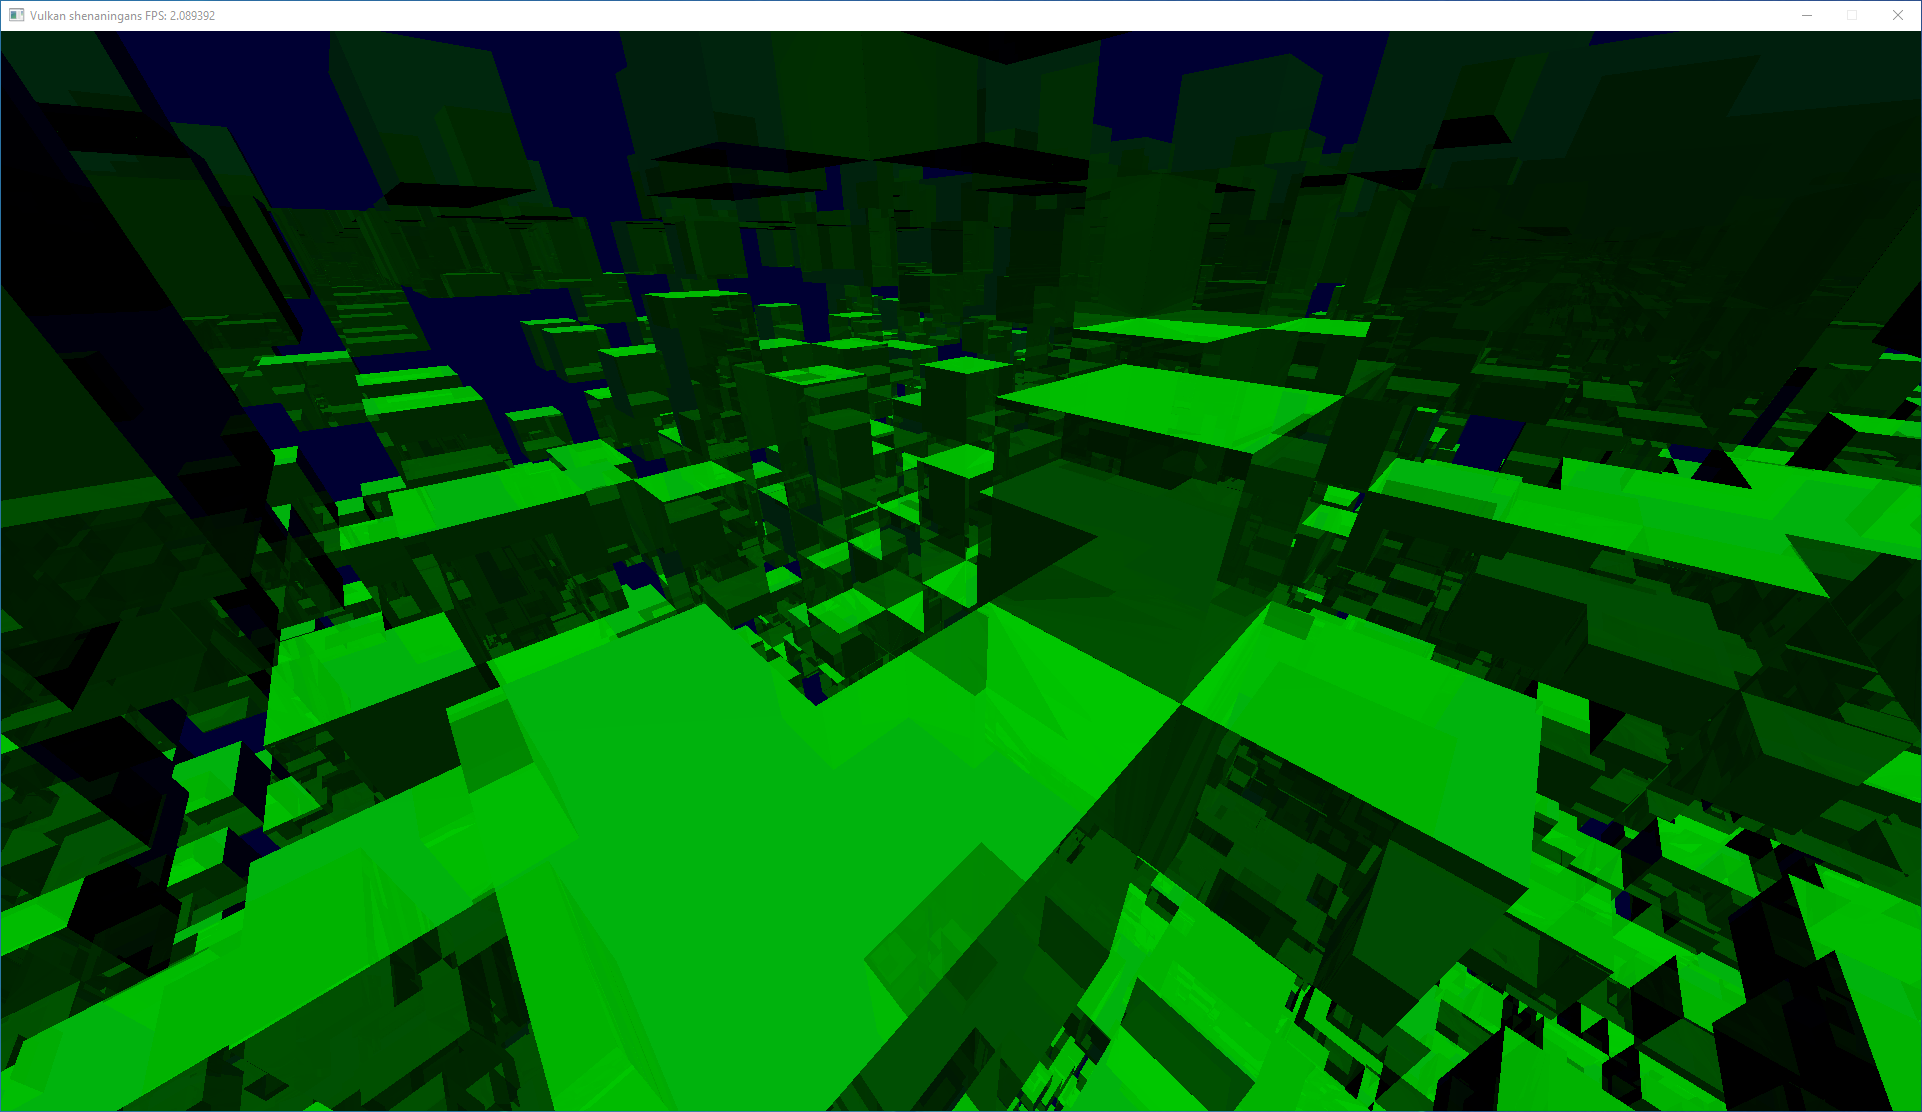
\includegraphics[width=1\textwidth]{tests/reflections_only.png}
\caption{Test with only reflections enabled}
\end{figure}
\end{center}

\begin{center}
\begin{figure}[H]
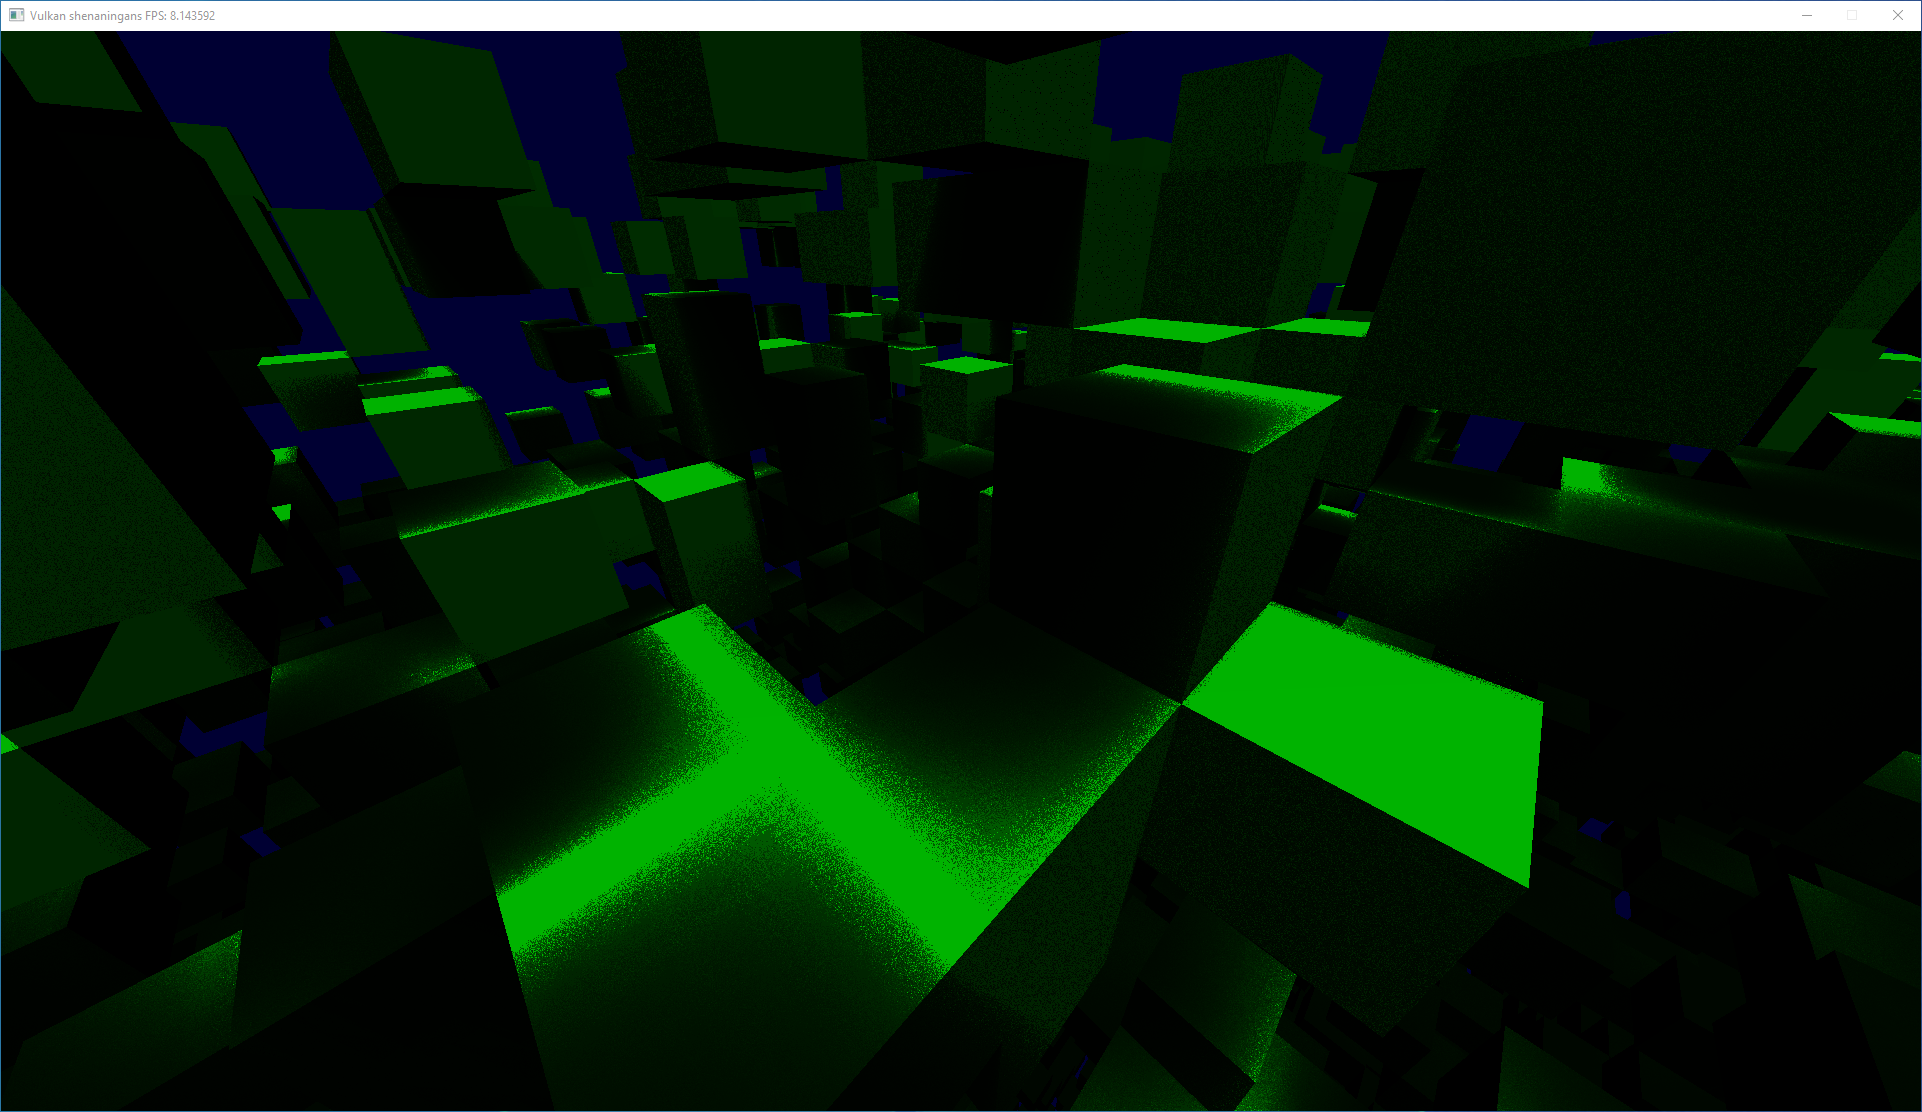
\includegraphics[width=1\textwidth]{tests/shadows_only.png}
\caption{Test with only shadows enabled}
\end{figure}
\end{center}

\begin{center}
\begin{figure}[H]
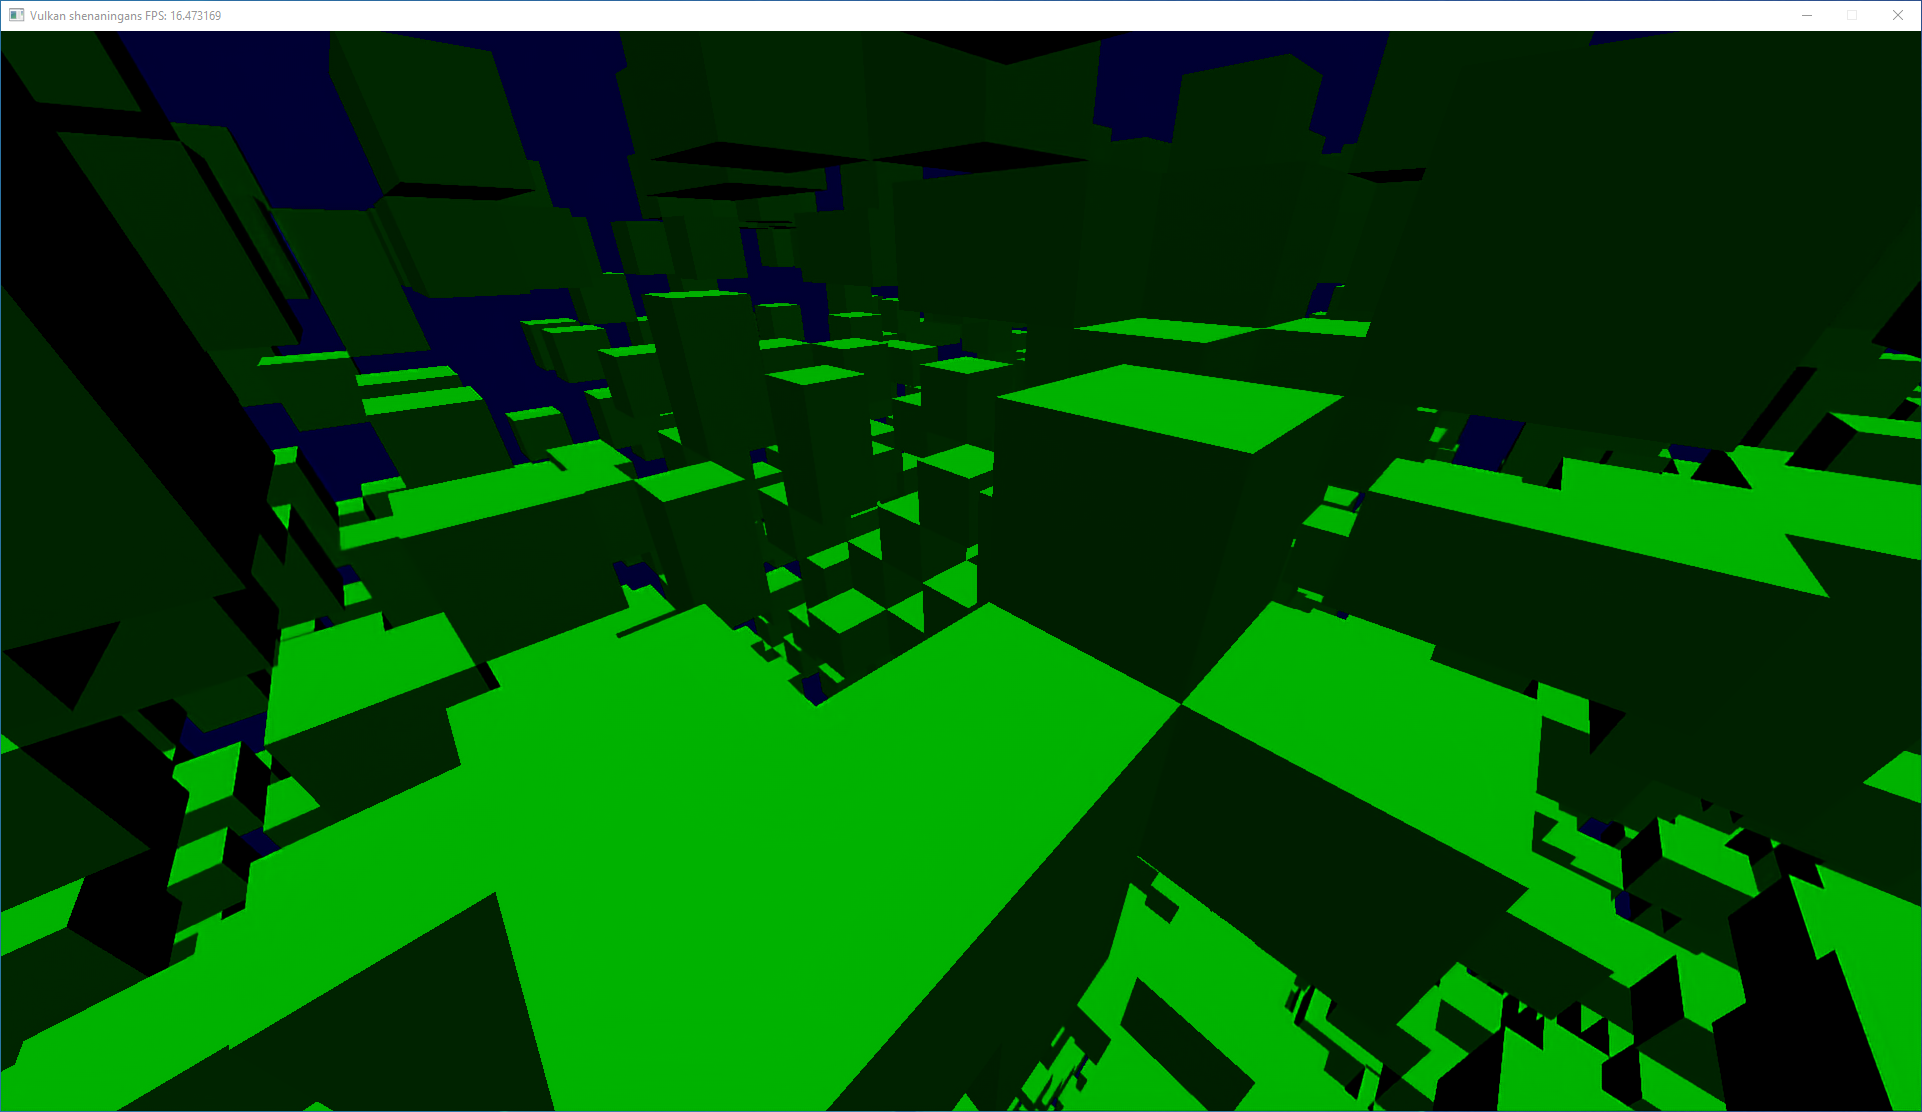
\includegraphics[width=1\textwidth]{tests/denoising_only.png}
\caption{Test with only denoising enabled}
\end{figure}
\end{center}

\begin{center}
\begin{figure}[H]
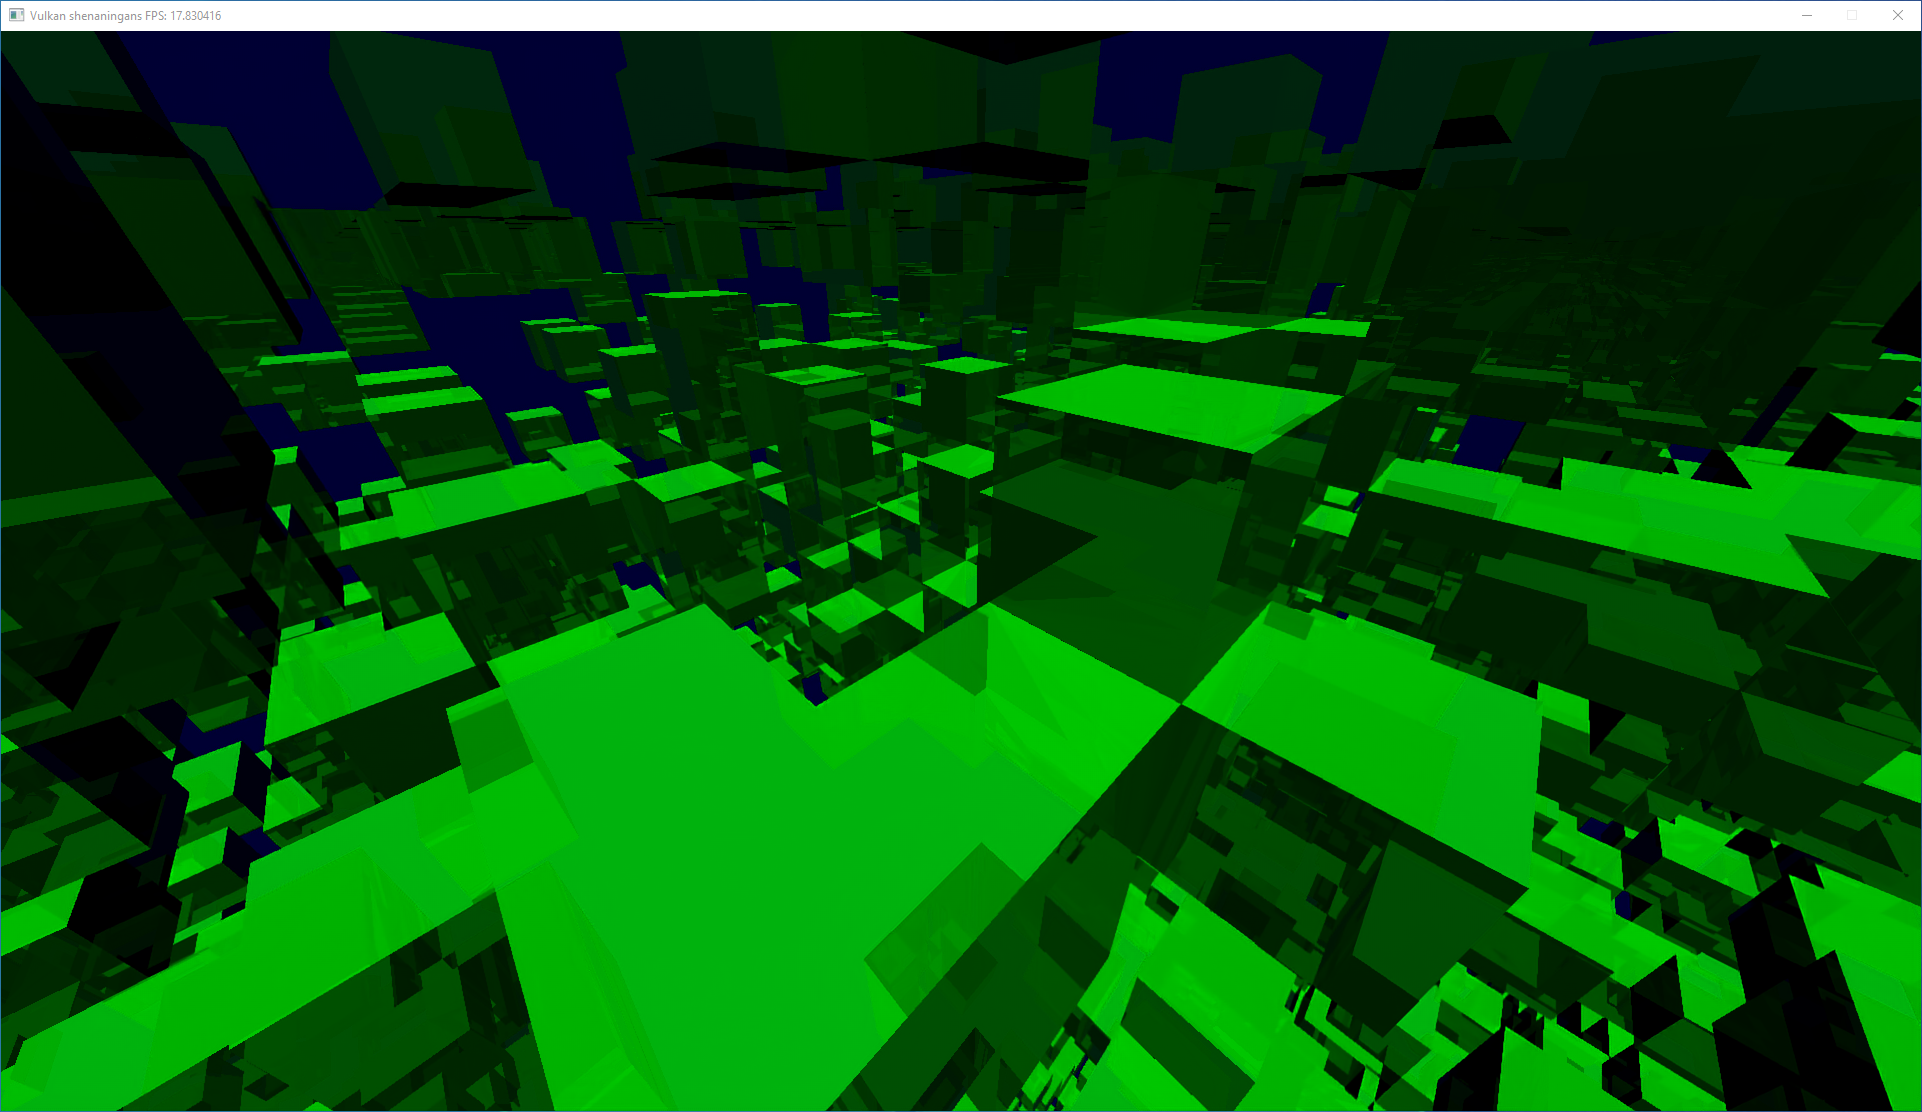
\includegraphics[width=1\textwidth]{tests/reflections+denoising.png}
\caption{Test with reflections and denoising}
\end{figure}
\end{center}

\begin{center}
\begin{figure}[H]
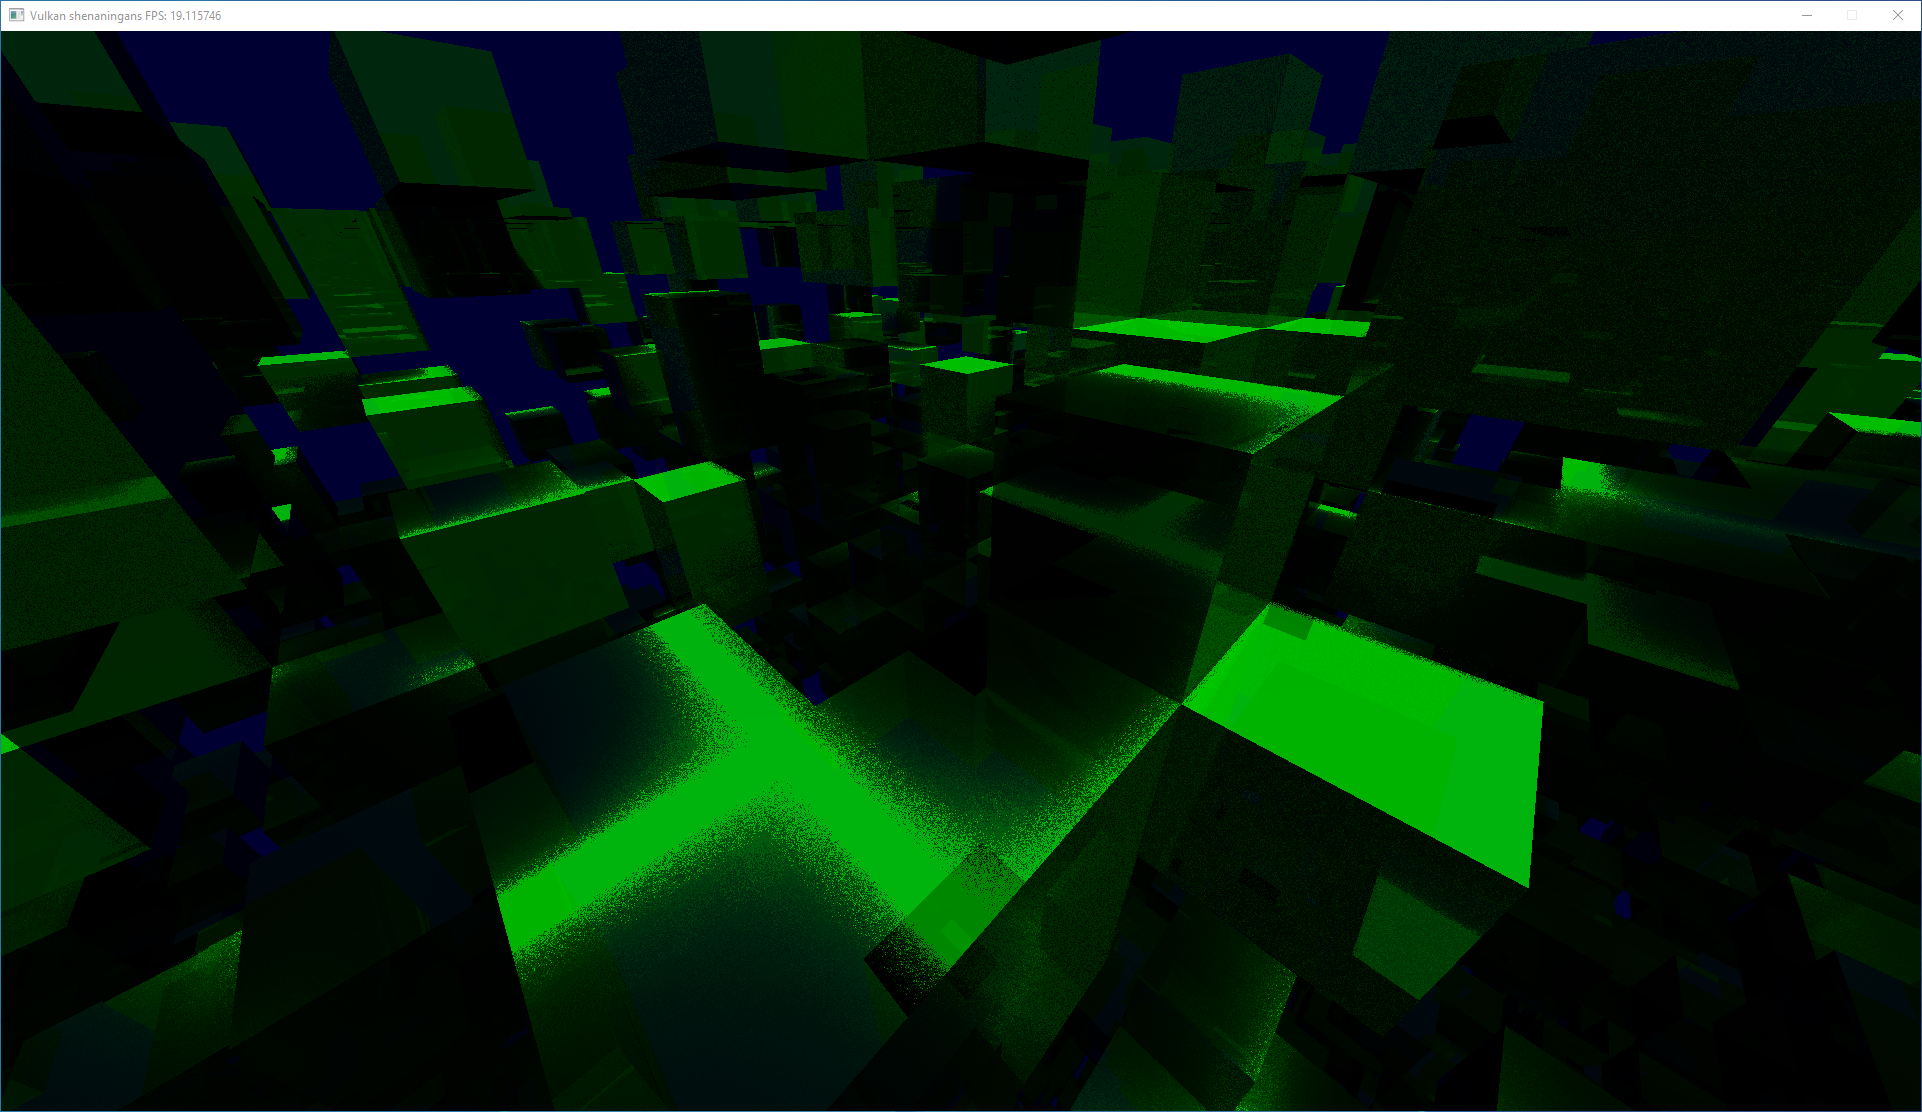
\includegraphics[width=1\textwidth]{tests/shadows+reflections.png}
\caption{Test with shadows and reflections}
\end{figure}
\end{center}

\begin{center}
\begin{figure}[H]
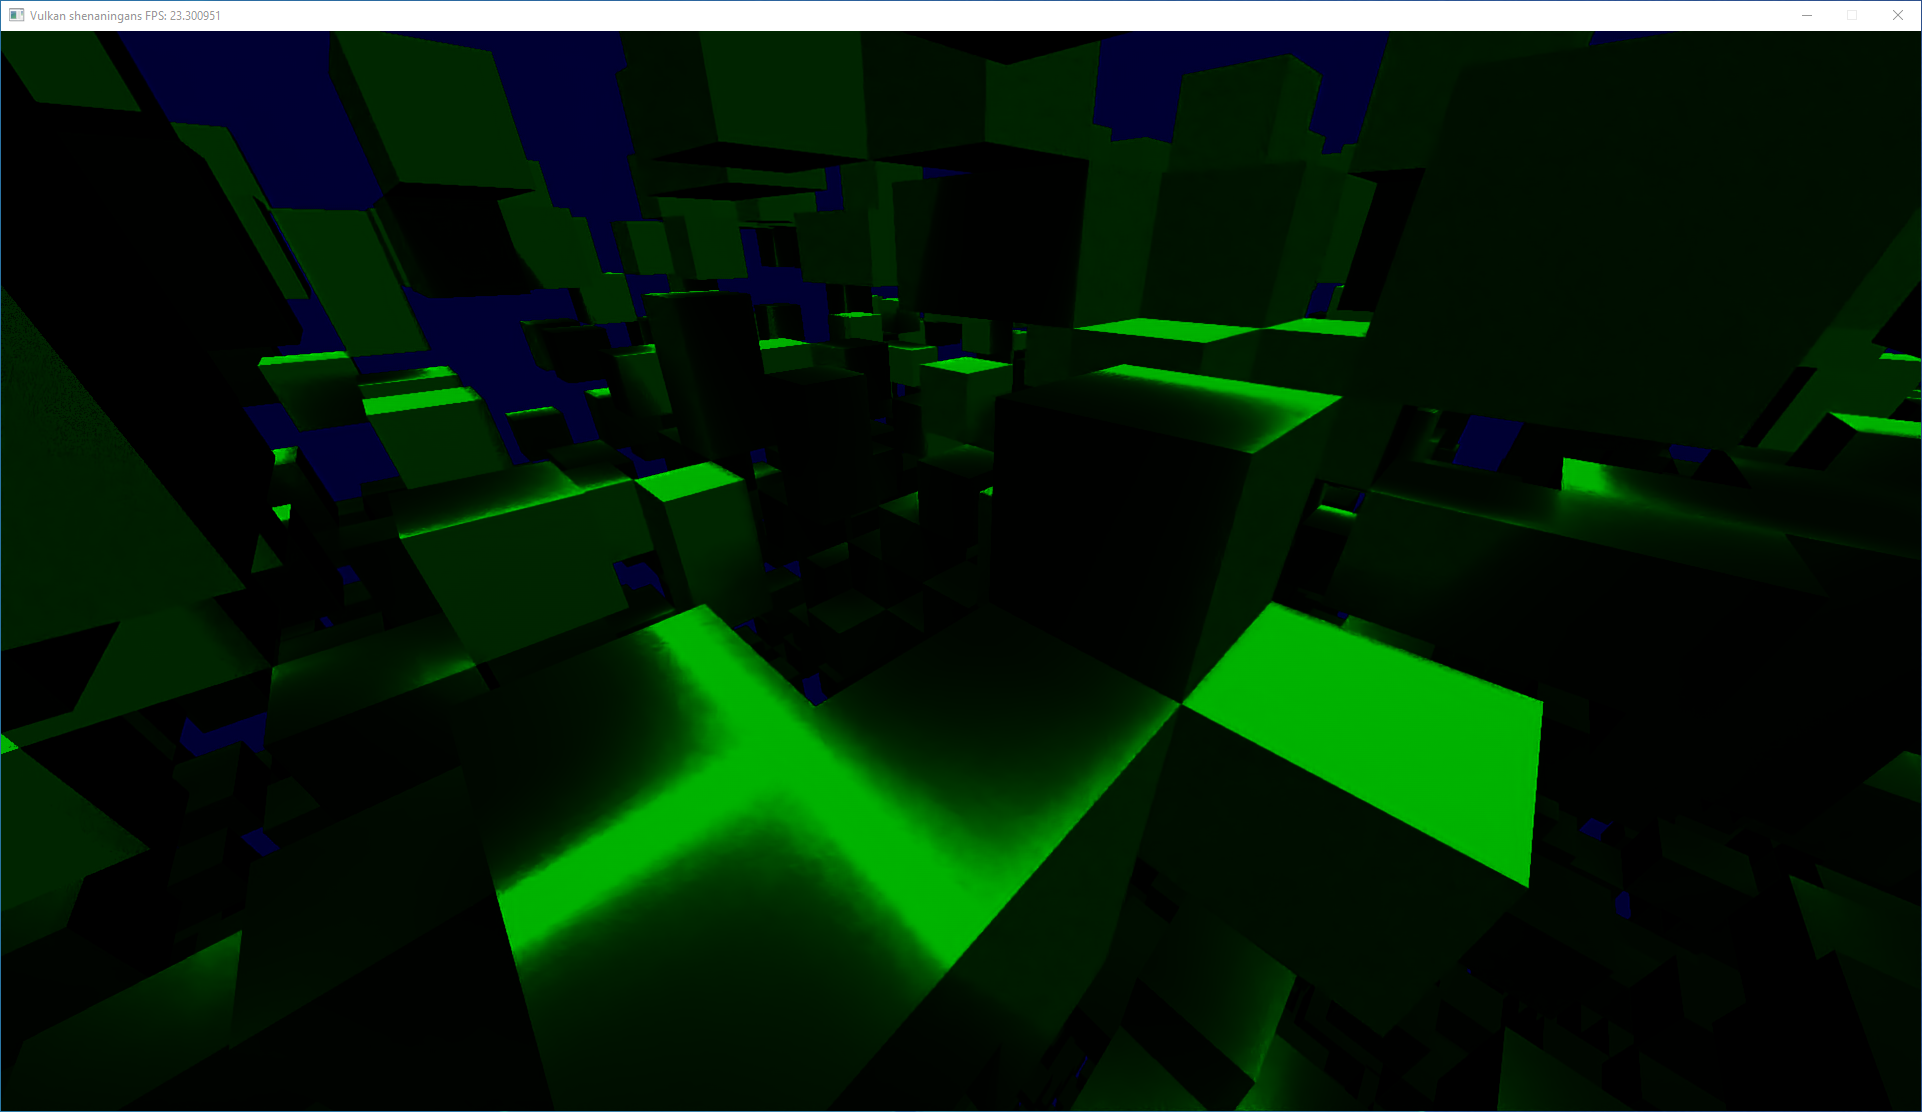
\includegraphics[width=1\textwidth]{tests/shadows+denoising.png}
\caption{Test with shadows and denoising}
\end{figure}
\end{center}

\begin{center}
\begin{figure}[H]
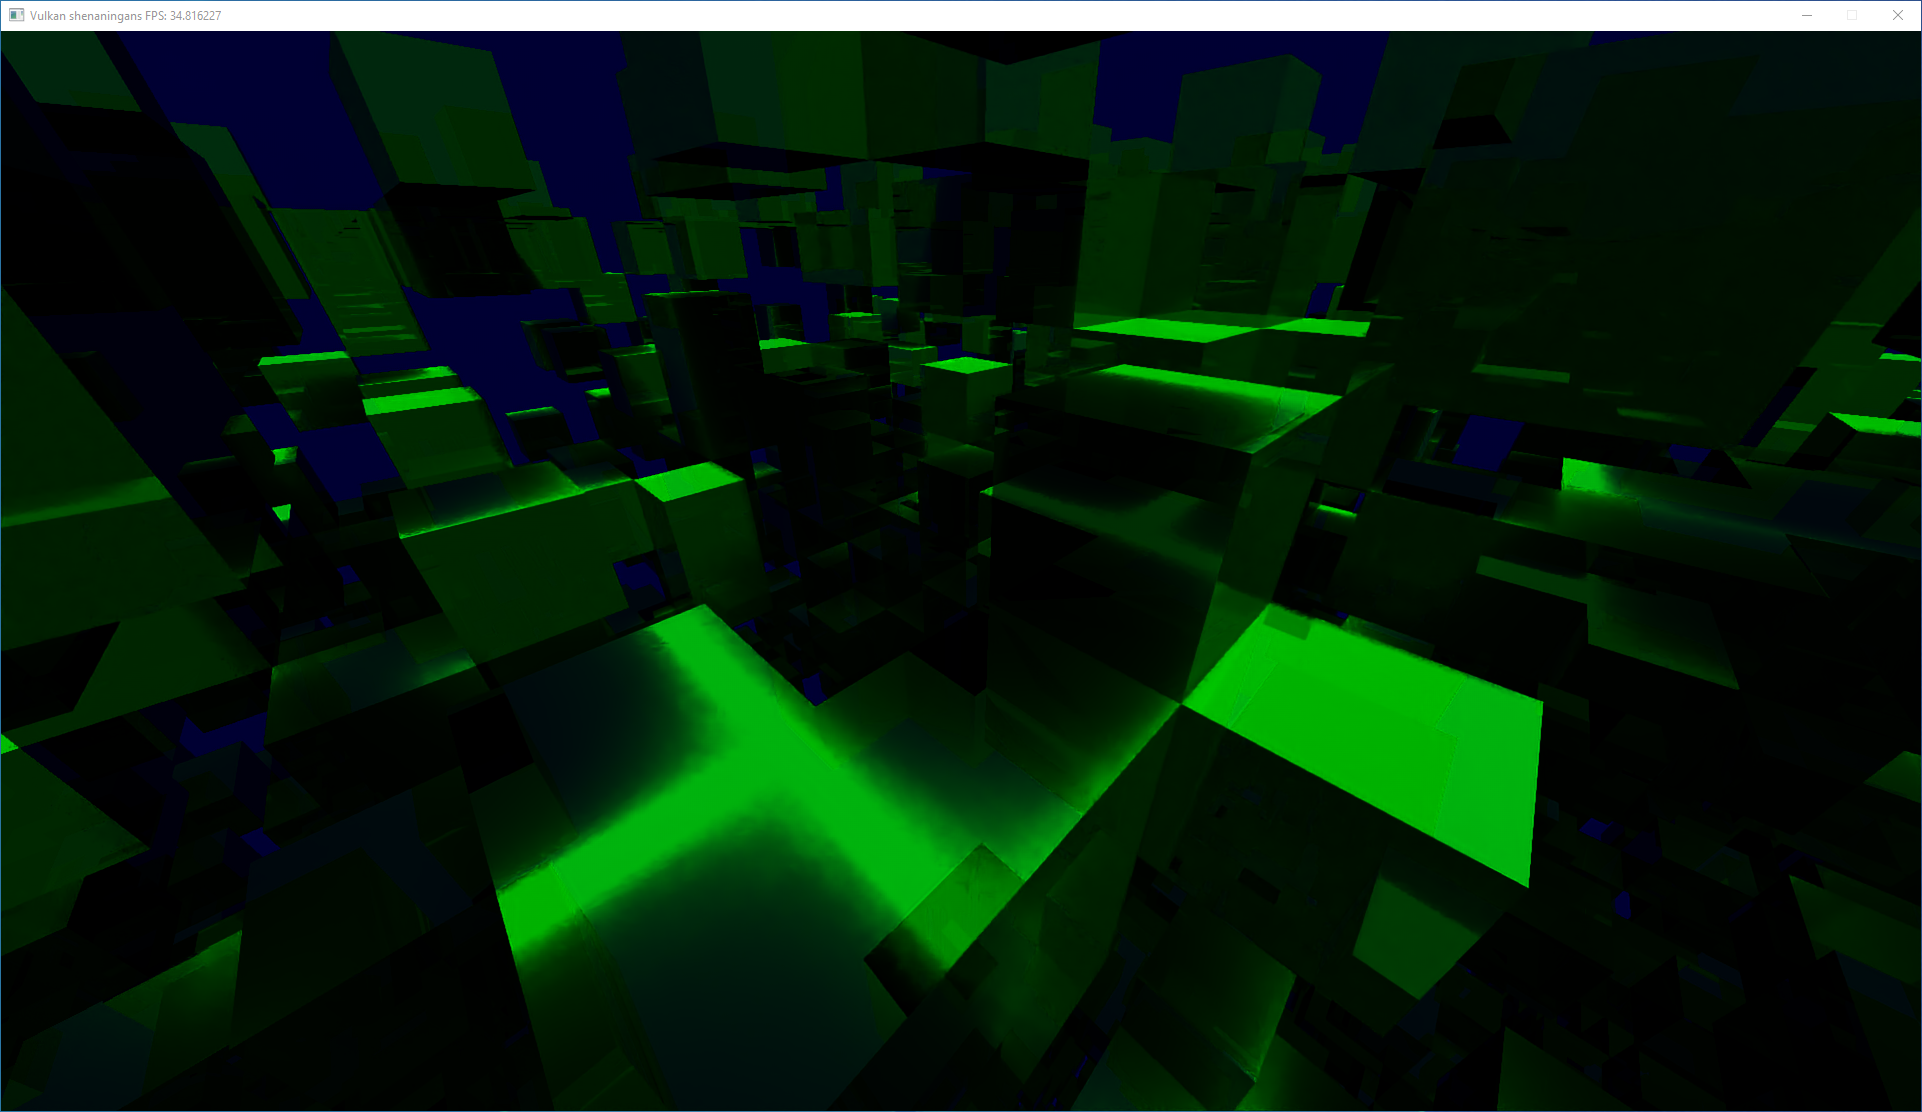
\includegraphics[width=1\textwidth]{tests/all_on.png}
\caption{Test with everything enabled}
\label{image:all_on}
\end{figure}
\end{center}

\section{Possible improvements and additions}
The application can be improved in several ways. Firstly, the greedy mesher, while meshing each of six slice sets concurrently, meshes them one chunk after another, and does so on only six concurrent threads at a time. The concurrent code is also only two times faster than the serial one, most likely due to the overhead of creating and destroying threads. The CPU also never goes above 40\% utilization, since it uses at most 37.5\% of threads available (on the test system). Using thread pools and generating all of the chunks in parallel could improve the performance significantly.
Greedy mesher is capable of processing chunks that are made of only two types of blocks. Enhancing it to be able to use an arbitrary number of block types should be relatively straightforward.

Light in the ray tracer is not attenuated, this feature could be implemented, but would require the redesign of the way colours are blended.

The ray tracer only works with a single light source. Adding more light sources would linearly increase the required number of rays per each intersection, so a different approach would be required. Instead of taking all of the samples of all of the lights, only a single sample could be taken per light source. This would still linearly increase the required number of rays per intersection, albeit a bit slower. A step further would be sampling only a certain amount of light sources per intersection and doing so only for light sources that are within a certain distance from the intersection.

\begin{center}
\begin{figure}[H]
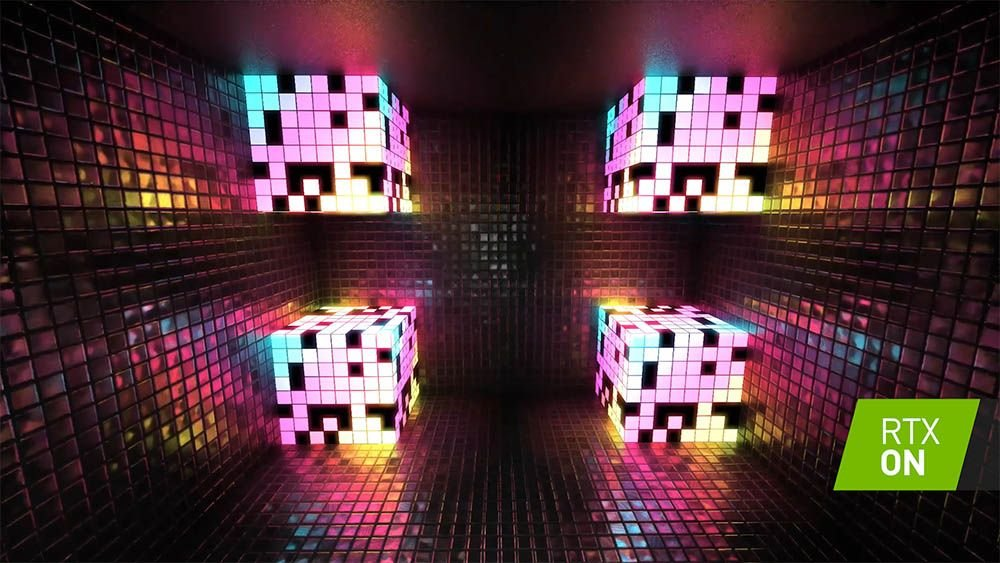
\includegraphics[width=1\textwidth]{rtx_on.jpg}
\caption{RTX in Minecraft \cite{minecraft_rtx}}
\end{figure}
\label{image:rtx_on}
\end{center}

The ray tracing model does not account for colour bleed from nearby surfaces which could be resolved similarly to shadows. Instead of a rectangular sample set, one would be derived from a hemisphere. Relatively short rays would be traced towards the sample points, blending the hit colours with the colour of the intersection.

Ambient occlusion could be implemented similarly to colour bleed, using hemispheres. Each ray would be fairly short and tested whether it hits the a nearby surface or not.

Denoiser currently only takes the ray tracing output image, but the API can also be given additional information in the form of an albedo and a normal render. A raster pipeline running parallel to the ray tracer could be set, writing this data to images that could then be passed to the denoiser along with the ray tracing output image, producing better results.

Currently, a scene is loaded at the start of the program and never changed. The application could be altered to load and unload chunks as the player moves through space. The time required to load the data from the disk and more importantly to build the accelerations structures on the fly would have to be taken into account.

Image 6.11 demonstrates what can be done with ray tracing when properly implemented. DirectX equvivalent of the Vulkan ray tracing extension was used to implement reflections, shadows and global illumination in Minecraft. DLSS is used to achieve playable framerates (>30FPS at 1080p on a GeForce RTX 2060 and above).


\chapter{Conclusion}
Ray tracing simplifies many concepts which, when using rasterization, need to be simulated by complex algorithms. When properly implemented, ray tracing produces soft shadows, accurate reflections and detailed global illumination, and does so inherently.

Its main drawback is its prohibitive cost - while GPUs today are technically capable of running the algorithm in real-time, they just are not fast enough to do everything we would like naively, requiring some kind of compromise:
\begin{itemize}
	\item limiting ray tracing to only certain aspects of the scene (only shadows, only reflections or only global illumination), while using rasterization for the rest
	\item ray tracing with a low number of samples per pixel, resulting in noisy images that needs to be denoised
	\item ray tracing at lower resolutions using one of the upscaling techniques to get the full resolution image
	\item accumulating lighting and other data over several frames, creating a higher quality renders, but with visible lighting latency and artefacts
\end{itemize}

The methods enumerated above are only a few possible optimizations and many implementations often use more than one of them. Especially interesting is rendering at a lower resolution and upscaling - Nvidia has been developing a deep learning powered technique called DLSS (Deep Learning Super Sampling) which runs in constant time but produces very good results.

However drastic the advancements in ray tracing have been in recent years, the (real-time) rendering industry has been using rasterization ever since GPUs were invented, developing the field for more than 30 years. With that in mind, it is abundantly clear that ray tracing will not be replacing rasterization in any foreseeable future. It will be used more often though, especially as more powerful hardware becomes available.

\bibliography{literatura}
\bibliographystyle{fer}

\newpage
\vspace*{\fill}
\thispagestyle{empty}
\begin{center}
{\bf Interaktivan prikaz vokseliziranog prostora s Vulkanom uz sklopovski ubrzano praćenje zrake}
\end{center}
\hspace*{\fill} {\bf Sa\v{z}etak} \hspace*{\fill} \par
\vspace*{25pt}

U ovom radu razrađen je prikaz konačnog vokseliziranog prostora upotrebom \linebreak sklopovski ubrzanog algoritma praćenja zrake. Uspoređena je standardna rasterizacija s algoritmom praćenja zraka te su opisani prednosti i mane jednog nad drugim. Posebna pažnja dana je načinu na koji Vulkan izlaže sklopovski ubrzano praćenje zrake kroz ekstenziju \texttt{VK\_KHR\_RAY\_TRACING}. Konačno, opisan je malen Vulkan primjer koji demonstrira osnovnu implementaciju algoritma praćenja zrake.

\kljucnerijeci{algoritam praćenja zrake, Vulkan, voksel, sklopovsko ubrzanje}

\engtitle{Rendering of Voxelized Space with Vulkan Using Hardware Accelerated Ray Tracing}
\begin{abstract}
This paper explores the real-time representation of finite voxelized space using hardware-accelerated ray tracing. It compares standard rasterization to ray tracing and outlines the benefits and drawbacks in comparison to each other. It explores how Vulkan exposes hardware ray tracing capabilities through its \texttt{VK\_KHR\_RAY\_TRACING} extension. Finally, a small Vulkan example is described that shows a basic implementation of the ray tracing algorithm.

\keywords{ray tracing, Vulkan, voxel, hardware acceleration}
\end{abstract}

\end{document}